\documentclass{article}
\usepackage{ctex}
\usepackage[utf8]{inputenc}
%\usepackage{natbib}
\usepackage[square,sort,comma,numbers]{natbib}
\usepackage{graphicx}
\usepackage{geometry}
\usepackage{booktabs}
\usepackage{siunitx}
\usepackage{listings}
\usepackage{subfigure}
\usepackage{appendix}
\usepackage{graphicx}
\usepackage{pythonhighlight}



\lstset{
    language=MATLAB,
    basicstyle=\ttfamily\small,
    aboveskip={1.0\baselineskip},
    belowskip={1.0\baselineskip},
    columns=fixed,
    extendedchars=true,
    breaklines=true,
    tabsize=4,
    prebreak=\raisebox{0ex}[0ex][0ex]{\ensuremath{\hookleftarrow}},
    frame=lines,
    showtabs=false,
    showspaces=false,
    showstringspaces=false,
    keywordstyle=\color[rgb]{0.627,0.126,0.941},
    commentstyle=\color[rgb]{0.133,0.545,0.133},
    stringstyle=\color[rgb]{01,0,0},
    numbers=left,
    numberstyle=\small,
    stepnumber=1,
    numbersep=10pt,
    captionpos=t,
    escapeinside={\%*}{*}
}

\usepackage{listings} % code display
\geometry{a4paper,centering,scale=0.8}
\usepackage[format=hang,font=small,textfont=it]{caption}
\usepackage[nottoc]{tocbibind}
\usepackage{float}
\usepackage{amsmath}

\usepackage[colorlinks=true, 
    linkcolor=blue,          % color of internal links
    citecolor=blue,        % color of links to bibliography
    filecolor=blue,      % color of file links
    urlcolor=blue]{hyperref}
    \usepackage[myheadings]{fullpage}

\numberwithin{equation}{subsection}
\newcommand{\HRule}[1]{\rule{\linewidth}{#1}}

\newcommand\degree{^\circ}
\date{}
%\bibliographystyle{plain}

\usepackage{abstract}
\setlength{\abstitleskip}{0em}%“摘要”与摘要正文间距
\renewcommand{\abstractnamefont}{\Large\bfseries}

\pagestyle{plain}

\geometry{a4paper,left=3cm,right=3cm}






\title{\heiti 基于微分方程与数值分析的波浪能最大功率设计}
%这里填写题目


\begin{document}
\maketitle
\vspace{-5em}%“摘要”与标题的间距



\begin{abstract}
波浪能装置是一种转化利用海洋能源的重要工具。在波浪的作用下,通过浮子与振子的相对运动驱使内部阻尼器做功,从而实现能量的转化输出。该装置在海水中的运动是一个复杂的过程,受到自身与外界多种因素的影响。实现波浪能装置的最大功率输出,对于发展利用可再生能源、应对环境污染问题均具有重大意义。
%第一段交代背景

\textbf{针对问题一:}构建浮子与振子垂荡时的物理模型。依据附件3和附件4提供的数据,结合附件1中波浪能装置的运动状态,分(1)与(2)两种情况分别对浮子与振子竖直方向上的运动进行受力分析。根据牛顿第二定律列出浮子与振子垂荡过程中的运动学\textbf{微分方程},通过换元整理转化为一阶显式常微分方程组。进而利用matlab中的\verb|odefun|函数求解微分方程的数值解,得到前40个波浪周期内时间间隔为$0.2s$的垂荡位移与速度。
%问题一摘要(\textbf{}加粗关键词)

\textbf{针对问题二:}在问题一垂荡位移与速度的建模基础上,利用附件3和附件4中参数数值,求得特定直线阻尼器阻尼系数下垂荡过程的相对位移与相对速度。将平均输出功率视为20个波浪周期至40个波浪周期内阻尼力做功量与用时的比值。而一段时间的做功量等于阻尼力对时间的积分,利用数值方法将其近似为微小梯形面积之和。(1)对于给定的较小步长,将直线阻尼系数在[0,100000]\textbf{遍历}(2)对于给定的较小的步长,将系数与幂指数在分别在[0,100000]与[0,1]之间\textbf{遍历}。得到平均输出功率的数据散点图,并通过最大值点的检索和估计,得到最大平均输出功率和对应阻尼系数。
%问题二摘要(\textbf{}加粗关键词)

\textbf{针对问题三:}构建浮子与振子垂荡纵摇时的物理模型。通过假定浮子的旋转轴以及其旋转轴心处的运动状态,利用附件3和附件4提供的数据,对浮子和振子在垂荡运动方向与纵摇旋转方向上进行受力分析。模型求解思路同问题一,将得到的运动方程化为一阶显式微分方程组后,进利用matlab中的\verb|odefun|函数求解微分方程的数值解,得到前40个波浪周期内时间间隔为$0.2s$的浮子与振子垂荡位移与速度、纵摇角位移与角速度。
%问题三摘要(\textbf{}加粗关键词)

\textbf{针对问题四:}在问题三的垂荡位移与速度、纵摇角位移与角速度的建模基础上,利用附件中参数值求得在给定直线阻尼系数与旋转阻尼系数下,垂荡纵摇过程中的相对位移与相对速度。建模思路同问题二,构建平均输出功率的数值求值模型。由于遍历耗时较长,选择增大搜索步长,转而利用\textbf{多重搜索}。逐次缩小区间以及步长,达到一定精度后,获取平均输出功率最大值以及其对应的最优阻尼系数。
%问题四摘要(\textbf{}加粗关键词)

\textbf{关键词:PTO;微分方程;遍历;多重搜索;数值解}

\end{abstract}

\newpage





{\centering\section{问题重述}}
随着经济和社会的发展,人类面临能源需求和环境污染的双重挑战,发展可再生能源产业已成为世界各国的共识。波浪能作为一种重要的海洋可再生能源,储量丰富,分布广泛,应用前景十分可观。实现波浪能的规模化利用,关键要提高波浪能装置的能量转换效率,保证能源获取效率。因此,设计最大输出功率的波浪能装置,对于发展利用可再生能源,应对环境污染问题具有重大意义。

图1(a)是一种波浪能装置示意图,由浮子、振子、中轴以及能量输出系统(PTO,包括弹簧和阻尼器)构成。振子、中轴及PTO被密封在浮子内部,浮子由质量分布均匀圆柱壳体和圆锥壳体组成,两壳体连接部分有一隔层。振子是穿在中轴上的圆柱体,通过PTO系统与中轴底座链接。在波浪的作用下,浮子运动并带动振子运动,通过二者的相对运动驱动阻尼器做功,将所做的功作为能量输出。

\begin{figure}[htbp]
    \centering
    \subfigure[直线阻尼器装置图]{
    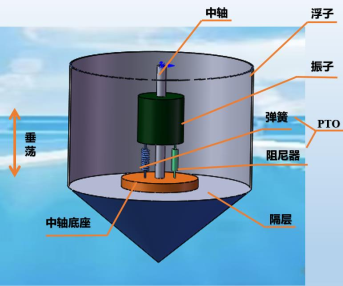
\includegraphics[scale=0.75]{波浪能装置图1.png} \label{1}
    }
    \subfigure[直线与旋转阻尼器装置图]{
    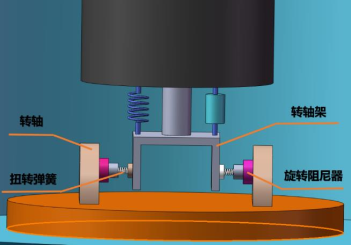
\includegraphics[scale=0.88]{波浪能装置图2.png} \label{2} 
    }
    \quad
    \caption{波浪能装置图}
\end{figure}
%插入子图拼图模板


\textbf{问题1:}在图1(a)的装置中,中轴底座固定于隔层的中心位置,弹簧和直线阻尼器一端固定在振子上,一端固定在中轴底座上,振子沿中轴做往复运动。直线阻尼器的阻尼力与浮子和振子的相对速度成正比,比例系数为直线阻尼器的阻尼系数。初始时刻浮子和振子平衡于静水中,海水作用的相关参数如附件3、4所示。现考虑浮子在波浪中只做垂荡运动,建立浮子与振子的运动模型,分别对以下两种情况计算浮子和振子在波浪激励力$f \cos \omega t$作用下,前$40$个波浪周期内时间间隔为$0.2s$的垂荡位移和速度:
(1)直线阻尼器阻尼系数为$10000\mathrm{N} \cdot \mathrm{s} / \mathrm{m}$
(2)直线阻尼器的阻尼系数与浮子和振子的相对速度的绝对值的幂成正比,其中比例系数取$10000$,幂指数取$0.5$.
    
\textbf{问题2:}仍考虑浮子在波浪中只做垂荡运动,利用附件3、4提供的参数值,分别对以下两种情况确定PTO系统的最大平均输出功率,以及直线阻尼器对应的最优阻尼系数:
(1)阻尼系数为常量,阻尼系数在区间$[0,100000]$内取值
(2)阻尼系数与浮子和振子的相对速度的绝对值的幂成正比,比例系数在区间$[0,100000]$内取值,幂指数在区间$[0,1]$内取值.

\textbf{问题3:}构建浮子与振子垂荡纵摇运动的物理模型。通过假定浮子的旋转轴以及其旋转轴心处的运动状态,利用附件3和附件4提供的数据,对浮子和振子在垂荡运动方向与纵摇旋转方向上进行受力分析。而后思路同问题一,化为一阶显式微分方程组后,进利用matlab中的\verb|odefun|函数求解微分方程的数值解,得到前40个波浪周期内时间间隔为$0.2s$的浮子与振子垂荡位移与速度,纵摇角位移与角速度。

\textbf{问题4:}仍考虑浮子在波浪中只做垂荡和纵摇运动。已知直线阻尼器和旋转阻尼器的阻尼系数均为常量且在区间$[0,100000]$内取值,结合附件3、4提供的参数值,计算PTO系统的最大输出功率及相应的最优阻尼系数。



%\begin{itemize}
%    \item 问题2:分析在问题1的双峰分峰模型中,峰高比对所建立的分峰模型的影响。除使用赛题提供数据外,可使用虚拟数据仿真协助分析。
 %   \item 问题3:利用附件2中三峰和四峰叠加的光谱曲线及数据,建立多个光谱峰叠加的复合光谱曲线模型,将多峰复合光谱曲线拆分为独立光谱曲线(最多四个峰),并给出分离后各峰的中心波长、高度及半峰宽,与其相应的准单色光谱进行比较。
%    \item 问题4:实际检测中的荧光光谱曲线多数是非对称的光谱曲线。利用附件3中实际的检测数据尝试建立非对称光谱曲线分峰的数学模型,将复合光谱曲线拟合拆分为对应的独立光谱曲线。
%\end{itemize}
%无序列表列出问题



{\centering\section{问题分析}}

\subsection{问题一的分析}
问题一要建立浮子与振子的运动模型,分两种情况讨论并求解前40个波浪周期内时间间隔为0.2s的垂荡位移和速度。由于浮子受到线性周期微幅波的作用,可近似认为海平面高度无变化,故选取海平面位置为零点,竖直向上为正方向建立坐标轴,对浮子与振子的运动进行定量化描述。结合附录3、4中的数据,对浮子与振子分别进行受力分析,得到描述二者位置变化的微分方程,换元整理得到等价的一阶显式微分方程组。进而利用matlab中的\verb|odefun|函数求解微分方程的数值解,得到所求时刻的垂荡位移与速度。%问题一分析内容
\subsection{问题二的分析}
问题二给出了阻尼系数的两种情况,要分别求解PTO系统的最大输出功率及对应的最优阻尼系数。首先根据平均功率的表达式构建数学模型,得到第一问中平均功率关于阻尼系数的函数,以及第二问中平均功率关于比例系数及幂指数的函数。对于给定的步长,将两个函数的自变量在区间范围内遍历,从而得到平均功率的数据散点图。观察散点图中的数据分布,对最大值点进行检索与估计,得到最大平均输出功率及对应的阻尼系数。
%问题二分析内容
\subsection{问题三的分析}
问题三要构建浮子与振子垂荡纵摇的运动模型,求解前40个波浪周期内时间间隔为0.2s的垂荡位移、垂荡速度、纵摇角位移、纵摇角速度。首先假定浮子旋转轴及其轴心处的运动状态,结合附件3、4中的数据,对浮子和振子在垂荡运动方向与纵摇运动方向上进行受力分析。再根据牛顿第二定律列出浮子与振子的运动学微分方程,通过换元整理转换为一阶显式微分方程。利用matlab中的\verb|odefun|函数求解微分方程的数值解,得到所求时刻的相关数据。
%问题三分析内容
\subsection{问题四的分析}
问题四要在问题三模型的基础上,求解给定参数范围内的最大平均输出功率及相应的阻尼系数。首先利用附件中参数求解在给定直线阻尼系数与旋转阻尼系数下,垂荡纵摇过程中的相对位移与相对速度。建模思路同问题二,继而构建平均输出功率的数值求值模型。由于直接进行高密度搜索需要的时间成本较高,这里采用多重搜索方法求解最大平均功率点。逐步缩小区间及步长,达到一定精度后,获得平均输出功率最大值及其对应的最优阻尼系数。
%问题四分析内容

\newpage

{\centering\section{模型假设}}

\begin{itemize}
    \item 假设一:海浪视为线性周期微幅波,不考虑海平面高度的变化。
    \item 假设二:浮子做纵摇运动时,始终绕着水平穿过重心的轴进行转动。
\end{itemize}
%无序列表列出问题假设
%这里也可以使用有序列表:
%\begin{enumerate}
%    \item 假设xxxxx
%    \item 假设xxxxx
%   \item 假设xxxxx
%\end{enumerate}



{\centering\section{符号说明}}

\begin{table}[H]
    \centering
    \begin{tabular}{ccc}%调整表格列数
        \toprule[1.5pt]%调节横线1粗细
        符号 & 解释 & 单位\\
        \midrule[1pt]%调节横线2粗细
        $m_{z}$&振子质量&$kg$\\
        $m_{x}$&浮子质量&$kg$\\
        $M$&附加质量&$kg$\\
        $k$&弹簧刚度&$N/m$\\
        $l$&弹簧原长&$m$\\ 
        $x_0$&浮子的初始位移&$m$\\
        $x$&浮子隔层圆心距海平面位移&$m$\\
        $x_g$&浮子重心距海平面位移&$m$\\
        $z$&振子底面圆心距海平面位移&$m$\\
        $z_p$&振子底面圆心距转轴中心位移&$m$\\
        $\alpha$&浮子和振子的相对角位移&$rad$\\
        $\beta$&浮子的角位移&$rad$\\
        $\eta _{\text{兴}}$&垂荡兴波阻尼系数&$N·s/m$\\
        $\eta_r$&旋转阻尼系数&$N·m·s$\\
        $\eta _{p}$&直线阻尼器阻尼系数&$N·s/m$\\
        $k_{\eta _{p}}$&直线阻尼器阻尼系数的比例系数&\\
        $k_r$&扭矩弹簧的刚度&$N·m/rad$\\
        $k_{\text{兴}}$&纵摇兴波阻尼系数&$N·m·s/rad$\\
        $k_{\text{恢}}$&静水恢复力矩系数&$N·m/rad$\\
        $f$&波浪激励力振幅&$N$\\ 
        $L$&波浪激励力矩振幅&$N·m$\\
        $\omega$&波浪频率&$s^{-1}$\\
        $J_f$&附加转动惯量&$kg·m^2$\\
        $\rho $&海水密度&$kg/m^3$\\
        $r$&浮子圆柱壳体半径&$m$\\
        $g$&重力加速度&$m/s^2$\\                      
         \bottomrule[1.5pt]%调节横线3粗细
    \end{tabular}}
    \caption{符号说明(注:未申明的变量以其在出现出的具体说明为准)}
\end{table}
%三线表,符号说明
%表格具体尺寸参数调整:https://blog.csdn.net/u010158659/article/details/78964030



{\centering\section{问题一模型的建立与求解}}

\subsection{模型建立}
题目将海浪视为线性周期微幅波,故海平面高度的变化可以忽略不计。选取海平面位置为零点,竖直向上为正方向建立坐标系。
规定浮子$x$隔层圆心的坐标表示浮子的位置,振子底面圆心的坐标$z$表示振子的位置。

\subsubsection{初始位置确定}

初始状态下,浮子与振子在静水中平衡,对整体受力分析得:
\begin{equation}
(m_x+m_z)g=\rho gV
\end{equation}

其中$V$表示浮子浸入水中的体积,代入附件4中数据解得:
$$V=\frac{m_x+m_z}{\rho }=7.12m^3$$

设$h_{\text{锥}}$表示浮子圆锥部分高度,则浮子圆锥部分体积为:
$$V_{\text{锥}}=\frac{1}{3} \pi r^2h_{\text{锥}}=0.84m^3,\quad V_{\text{锥}}<V$$

此时浮子的圆锥部分完全浸入水中,计算浮子的初始位置得:
\begin{equation}
    x_0=-\left(\frac{V-V_{\text{锥}}}{\pi r^2}+h_{\text{锥}}\right)=-2.00(m)
\end{equation}

\subsubsection{第一小问模型建立}
已知直线阻尼器的阻尼系数$\eta _{p}=10000 N·s/m$。初始状态下,浮子圆锥部分未露出水面。由于运动的连续性,浮子在开始运动的一段时间内,圆锥部分仍位于水面之下。在浮子开始运动至圆锥部分未出水的时段,选取任意时刻分析浮子与振子的运动状态。
\begin{equation}
\left\{\begin{array}{l}
   \text{浮子受到的浮力:}F_{11}=m_{x} g +m_{z} g+\rho g \pi r^{z}\left(x_{0}-x\right)\\
   \text{浮子受到的重力:}F_{12}=-m_{x} g\\
   \text{浮子受到的波峰激励力:}F_{14}=f \cos \omega t\\
   \text{浮子受到的兴波阻尼力:}F_{15}=-\eta_{\text{兴}} \dot{x}\\
   \text{浮子受到的弹簧与阻尼器作用力:}F_{16}=-k\left(l_{0}-z+x\right)-\eta_{p}(\dot{x}-\dot{z})\\
\end{array}\right.
\end{equation}

根据牛顿第二定律,$F_{11}+F_{12}+F_{13}+F_{14}+F_{15}=(m_x+M)\ddot{x}$,整理得:
\begin{equation}
m_{z} g+\rho g \pi r^{z}\left(x_{0}-x\right)+f \cos \omega t-\eta_{\text{兴}} \dot{x}-k\left(l_{0}-z+x\right)-\eta_{p}(\dot{x}-\dot{z})=\left(m_{x}+M\right) \ddot{x}
\end{equation}

\begin{equation}
\left\{\begin{array}{l}
    \text{振子受到的重力:}F_{16}=-m_{z} g\\
    \text{振子受到的弹簧与阻尼器作用力:}F_{17}=k\left(l_{0}-z+x\right)+\eta_{p}(\dot{x}-\dot{z})
\end{array}\right.
\end{equation}

根据牛顿第二定律,$F_{16}+F_{17}=m_{z} \ddot{z}$,整理得:
\begin{equation}
k\left(l_{0}-z+x\right)+\eta_{p}(\dot{x}-\dot{z})-m_{z} g=m_{z} \ddot{z}
\end{equation}

整理方程(5.1.4),(5.1.6),换元$\dot{x}=v_{x},\dot{z}=v_{z} $,得一阶显式微分方程组:
\begin{equation}
\left\{\begin{array}{l}
    \dot{x}=v_{x}\;,\; \dot{z}=\v_{z} \\
    \left(m_{x}+m\right) \dot{v}_{x}=m_{z} g+\rho g x^{2}\left(x_{0}-x\right)+f \cos (w t)-\eta_{\text{兴}} v_{x}-k\left(l_{0}-z+x\right)-\eta_{p}\left(v_{x}-v_{z}\right) \\
    m_{z} \dot{v}_{z}=k\left(l_{0}-z+x\right)+\eta_{p}\left(v_{x}-v_{z}\right)-m_{z} g .
\end{array}\right.
\end{equation}

\subsubsection{第二小问模型建立}
已知直线阻尼器的阻尼系数$\eta _{p}=k_{\eta _{p}}|{v_x}-{v_z}|^{\frac{1}{2}}$,比例系数$k_{\eta _{p}}=10000$。参照5.1.2,在浮子开始运动至圆锥部分未出水的时段,选取任意时刻分析浮子与振子的运动状态。相较第一小问,此问仅有阻尼系数$\eta _p$发生变化。只需将$\eta _{p}$的表达式带入(5.1.7),可得问题二的显式微分方程组:
\begin{equation}
    \left\{\begin{array}{l}
        \dot{x}=v_{x}\;,\; \dot{z}=\v_{z} \\
        \left(m_{x}+m\right) \dot{v}_{x}=m_{z} g+\rho g x^{2}\left(x_{0}-x\right)+f \cos (w t)-\eta_{\text{兴}} v_{x}-k\left(l_{0}-z+x\right)-k_{\eta _{p}}|{v_x}-{v_z}|^{\frac{1}{2}}\left(v_{x}-v_{z}\right) \\
        m_{z} \dot{v}_{z}=k\left(l_{0}-z+x\right)+k_{\eta _{p}}|{v_x}-{v_z}|^{\frac{1}{2}}\left(v_{x}-v_{z}\right)-m_{z} g .
    \end{array}\right.
    \end{equation}



\subsection{模型求解}

\subsubsection{第一小问模型求解}
调用matlab中的\verb|odefun|函数求解方程组(5.1.7)的数值解(程序见附录A.1)。以0.2s为步长得到各时刻浮子与振子的位置坐标及速度。以红色点表示振子,蓝色点表示浮子,绘制散点图如下:

\begin{figure}[H]
    \centering
    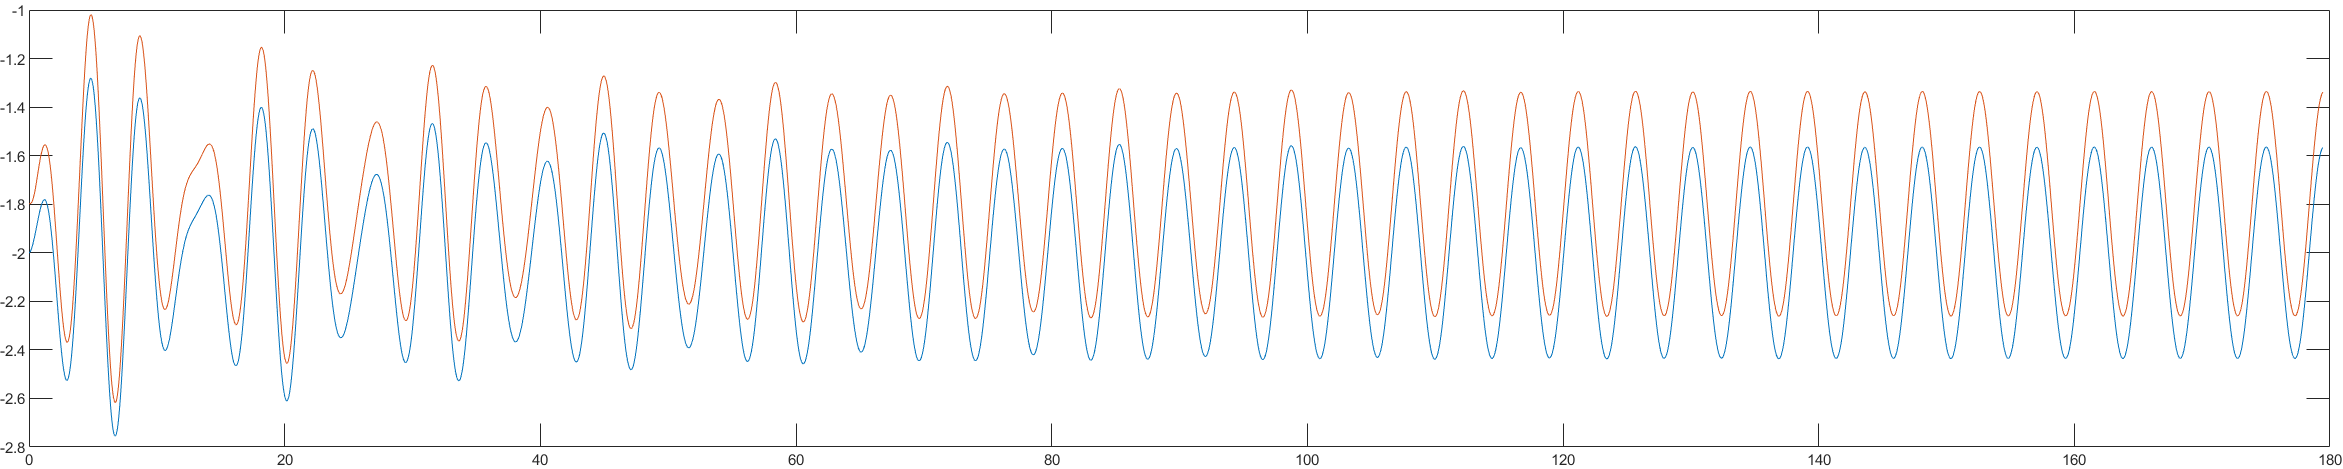
\includegraphics[scale=0.3]{问题1-1位移.png}
    \caption{问题1-1位置与时间关系图}
\end{figure}
%插入单张图片
\begin{figure}[H]
    \centering
    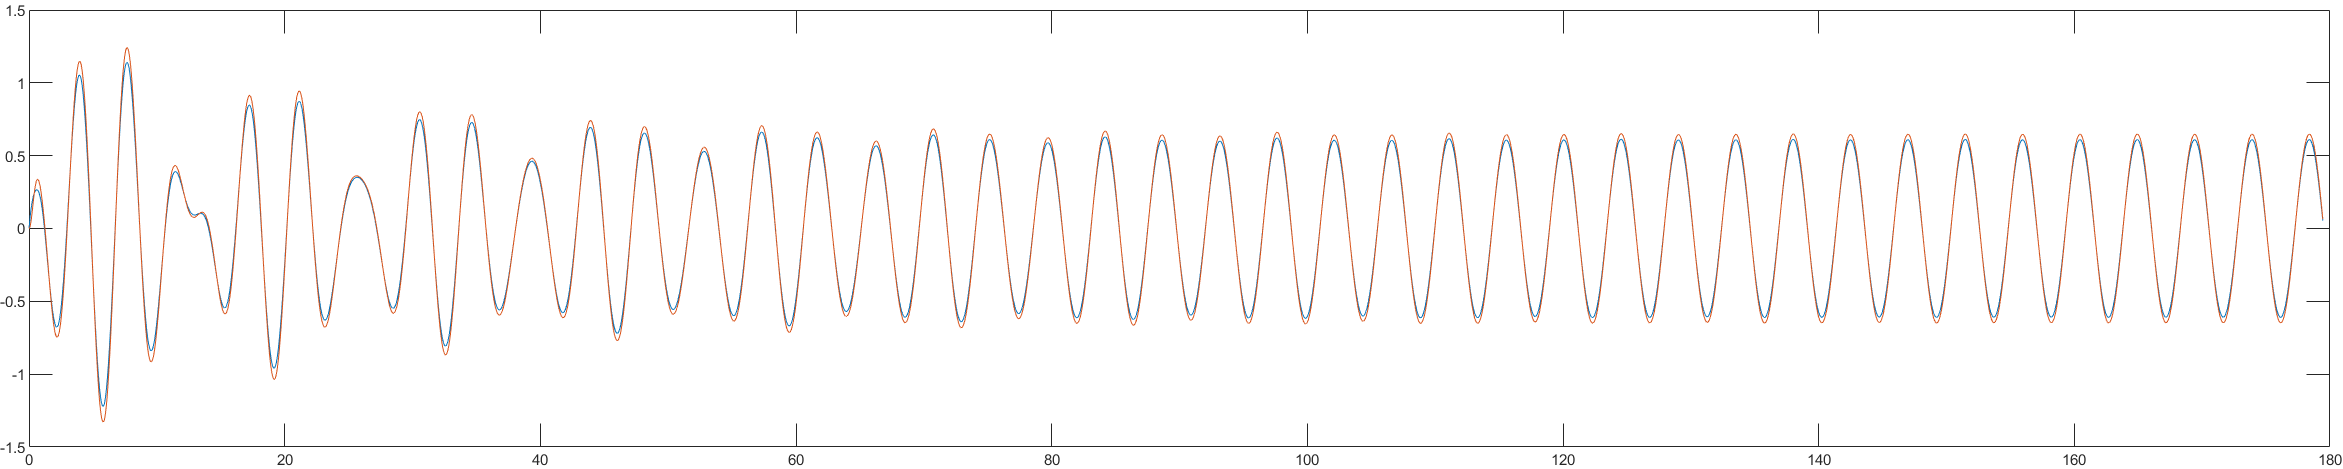
\includegraphics[scale=0.3]{问题1-1速度.png}
    \caption{问题1-1速度与时间关系图}
\end{figure}
%插入单张图片

在建模过程中,我们仅描述了浮子开始运动至圆锥部分未出水时段中任意时刻的运动状态。由浮子位置与时间关系图可知,此阶段运动中浮子圆锥部分并未露出水面。由运动的连续性可以推得,浮子垂荡运动全程圆锥部分均不会露出水面,模型求解得到的结论数据即为浮子与振子的全程运动数据。将得到的位置坐标转换为位移量,与速度数据共同存储于result1-1.xlsx文件中,提取10 s、20 s、40 s、60 s、100 s时刻数据如下表:

\begin{table}[!htbp]
    \centering
    \begin{tabular}{|c|c|c|c|c|}\hline
        时间(s) &浮子位移(m)&浮子速度(m/s)&振子位移(m)&振子速度(m/s)\\\hline
        10&-0.19

        &-0.64

        &-0.21

        &-0.69

        \\
        20&-0.59

        &-0.24

        &-0.63

        &-0.27

        \\
        40&0.29

        &0.31

        &0.30

        &0.33

        \\
        60&-0.31

        &-0.48

        &-0.33

        &-0.52

        \\
        100&-0.08

        &-0.60

        &-0.08

        &-0.64

        \\
        \hline
    \end{tabular}
    \caption{问题1-1结论数据}
\end{table}
%表格具体尺寸参数调整:https://blog.csdn.net/u010158659/article/details/78964030

\subsubsection{第二小问模型求解}
调用matlab中的\verb|odefun|函数求解方程组(5.1.8)的数值解(程序见附录A.2)。以0.2s为步长得到各时刻浮子与振子的位置坐标及速度。以红色点表示振子,蓝色点表示浮子,绘制散点图如下.
\begin{figure}[H]
    \centering
    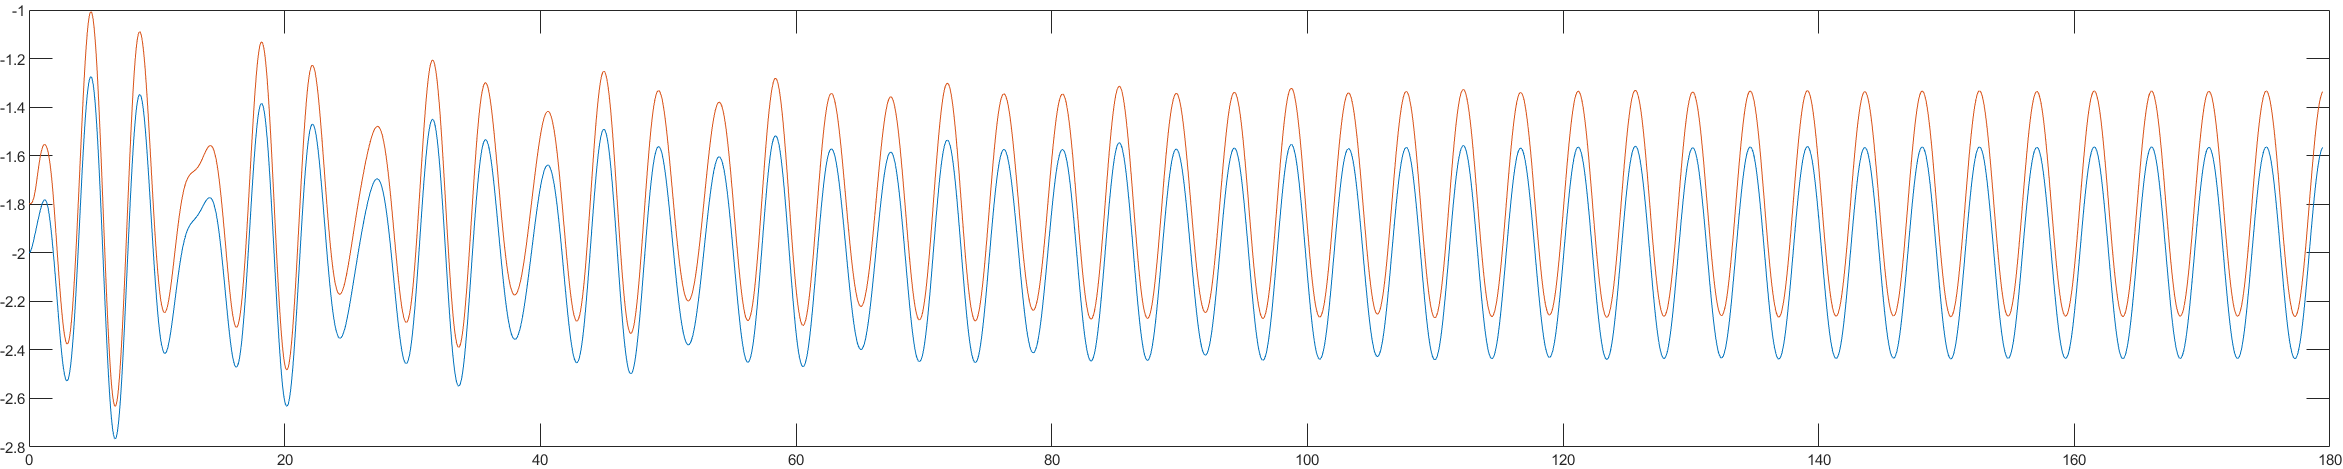
\includegraphics[scale=0.3]{问题1-2位移.png}
    \caption{问题1-2位置与时间关系图}
\end{figure}
%插入单张图片
\begin{figure}[H]
    \centering
    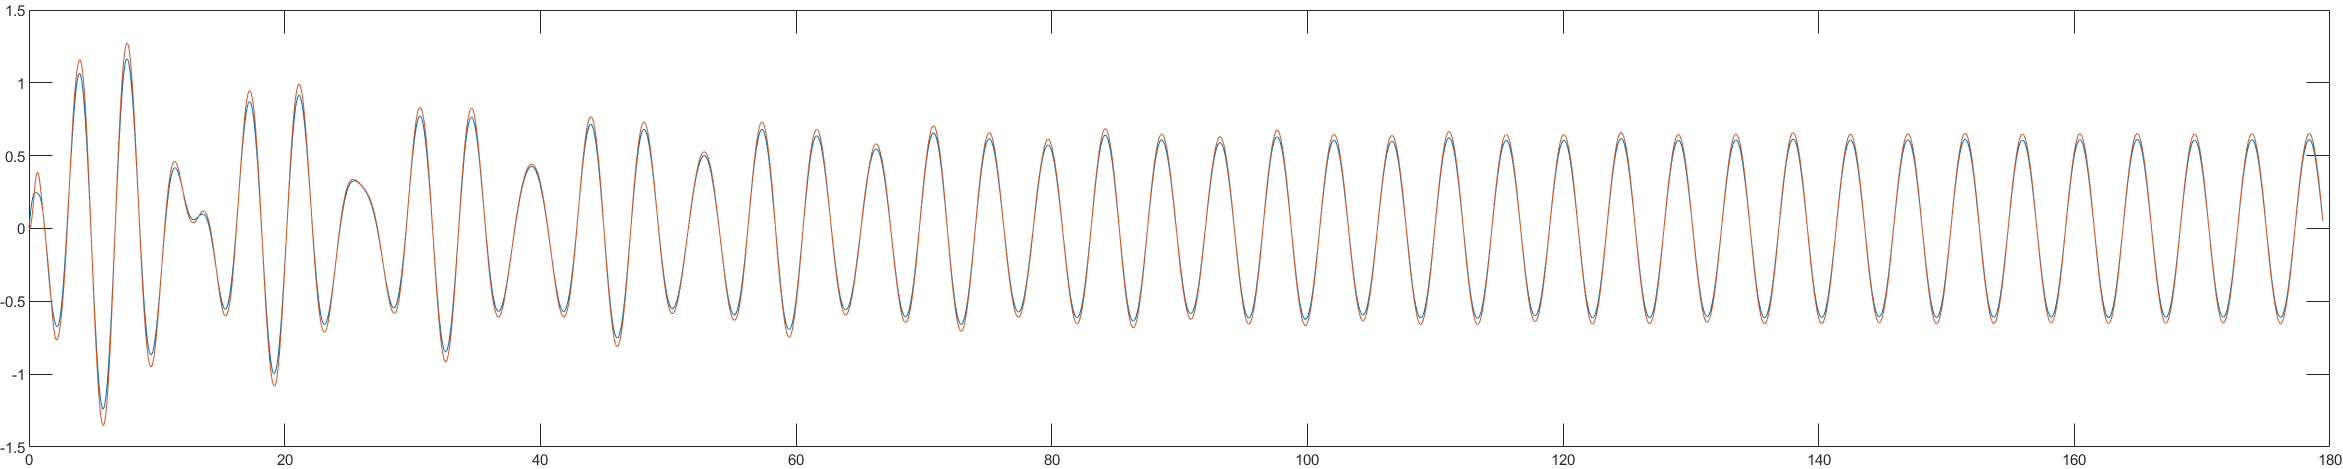
\includegraphics[scale=0.3]{问题1-2速度.png}
    \caption{问题1-2速度与时间关系图}
\end{figure}
%插入单张图片

同5.2.1,由运动连续性可以推得浮子垂荡运动全程圆锥部分均不会露出水面,模型求解得到的数据即为浮子与振子全程运动数据。将得到的位置坐标转换为位移量,与速度数据共同存储于result1-2.xlsx文件中,提取10 s、20 s、40 s、60 s、100 s时刻数据如下表:


\begin{table}[!htbp]
    \centering
    \begin{tabular}{|c|c|c|c|c|}\hline
        时间(s) &浮子位移(m)&浮子速度(m/s)&振子位移(m)&振子速度(m/s)\\\hline
        10&-0.21&	-0.65	&-0.23	&-0.70
        \\
        20&-0.61&	-0.25	&-0.66	&-0.28

        \\
        40&0.27	&0.30&	0.28&	0.31

        \\
        60&-0.33	&-0.49&	-0.35&	-0.52

        \\
        100&-0.09&	-0.61&	-0.09&	-0.65

        \\
        \hline
    \end{tabular}
    \caption{问题1-2结论数据}
\end{table}
%表格具体尺寸参数调整:https://blog.csdn.net/u010158659/article/details/78964030



{\centering\section{问题二模型的建立与求解}}

\subsection{模型建立}
推导PTO系统平均功率表达式可得:
$$
P=\frac{\Delta W}{\Delta t}=\frac{1}{\Delta t} \int_{t_{0}}^{t_{1}} F_{\text{阻尼}} d(x-z)
$$

由于两种情况下阻尼系数$\eta _p$表达式不同,针对两种不同的$F_{\text{阻力}}$分别建模如下.

\subsubsection{第一小问模型建立}
已知阻尼系数为常量且在区间$[0,10000]$内取值,此时$F_{\text{阻力}}=\eta_{p}\left(v_{x}-v_{z}\right)$,则有:
\begin{equation}
\Delta w=\int_{t_{0}}^{t_{1}} \eta_{p}\left(v_{x}-v_{z}\right) d(x-z) =\int_{t_{0}}^{t_{1}} \eta_{p}\left(v_{x}-v_{z}\right)^{2} d t =\eta_{p} \int_{t_{0}}^{t_{1}}\left(v_{x}-v_{z}\right)^{2} d t .
\end{equation}

浮子刚开始运动的一段时间内,平衡状态与周期性可能不稳定。为了避免这种不稳定对平均功率的求解造成影响,考虑选取第20个波浪周期至第40个波浪周期作为求解时段。即取$ t_{0}=20 \times \frac{2 \pi}{\omega}, \quad t_{1}=40 \times \frac{2 \pi}{\omega}$,设$\Delta t=t_1-t_0$,使用数值积分的梯形积分法求解平均功率,得到平均功率$P$关于阻尼系数$\eta _{p}$的函数表达式:
\begin{equation}
P=\frac{1}{\Delta t} \eta_{p}\int_{t_0}^{t_{1}}\left(v_{x}-v_{z}\right)^{2} d t \approx \frac{1}{\Delta t} \eta_{p}\sum\limits_{i=1}^{n-1} \frac{\Delta v_{x z}^{2}(i+1)+\Delta v_{x z}^{2}(i)}{2} h
\end{equation}

其中$\left(v_{x}-v_{z}\right)^{2}=\Delta v_{x z}^{2},\; h=0.2s $.

\subsubsection{第二小问模型建立}
已知阻尼系数表达式为$\eta _{p}=k_{\eta _{p}}|{v_x}-{v_z}|^{\alpha}$,其中$k_{\eta _{p}}$在区间$[0,100000]$内取值,$\alpha$在区间$[0,1]$内取值。参照6.1.1,选取第20个波浪周期至第40个波浪周期作为求解时段,取$ t_{0}=20 \times \frac{2 \pi}{\omega}, \quad t_{1}=40 \times \frac{2 \pi}{\omega}$。相较第一小问,此问仅有阻尼系数$\eta_p$发生变化,只需将$\eta_p$的表达式代入(6.1.2),得到平均功率$P$关于比例系数$k_{\eta_{p}}$与幂指数$\alpha$的函数表达式:
\begin{equation}
    P=\frac{1}{\Delta t} k_{\eta _{p}}\int_{t_0}^{t_{1}}|{v_x}-{v_z}|^{\alpha+2} d t \approx \frac{1}{\Delta t} k_{\eta _{p}} \sum\limits_{i=1}^{n-1} \frac{\Delta v_{x z}^{\alpha+2}(i+1)+\Delta v_{x z}^{\alpha+2}(i)}{2} h
\end{equation}
    
其中$|v_{x}-v_{z}|^{\alpha+2}=\Delta v_{x z}^{2},\; h=0.2s $.
    

\subsection{模型求解}

\subsubsection{第一小问模型求解}
已知平均功率$P$是关于阻尼系数$\eta _p$的函数,定义域区间$[0,100000]$。对区间$[0,100000]$以$10$为步长做遍历,便可得到不同阻尼系数对应的平均功率数据。整理数据绘制散点图见图6(a),遍历数据点用蓝色表示。

\begin{figure}[htbp]
    \centering
    \subfigure[遍历数据散点图]{
    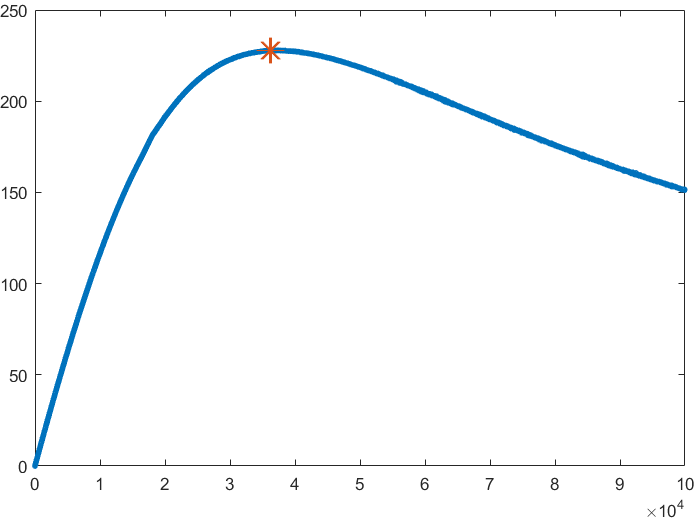
\includegraphics[scale=0.3]{问题2-1整体.png} \label{1}
    }
    \subfigure[最大值点检索结果]{
    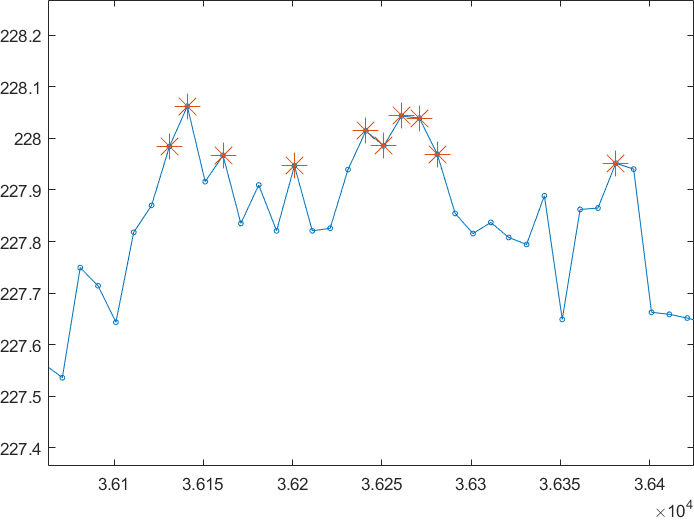
\includegraphics[scale=0.3]{问题2-1局部.png} \label{2} 
    }
    \quad
    \caption{问题2-1$\;\,p-\eta _p$散点图}
\end{figure}

检索遍历数据中平均功率最大的10个点,在图中用红色星号标出。对图6(a)局部放大得到图6(b),观察10个最大值点的位置分布。由检索数据可知(程序见附录B.1):10个最大值点对应的功率极差小于$0.21W$,不足平均值$227.9963W$的千分之一;对应的阻尼系数极差小于$300$,不足平均值$36232$的百分之一,不足区间长度$100000$的千分之三。10个最大值点分布较为密集,故采用10组数据的平均值表示求解结果,得到最大功率与阻尼系数的近似值。

\textbf{【结论】}最大平均功率$P_{max}=227.9963W$,对应阻尼系数$\eta _p =36232N·s/m$.


\subsubsection{第二小问模型求解}
已知平均功率是关于比例系数$k_{\eta _{p}}$与幂指数$\alpha$的函数,定义域$k_{\eta _p}\in [0,100000],\;\alpha\in[0,1]$,对区间$[0,100000]$以500为步长做遍历,对区间$[0,1]$以0.025为步长做遍历,得到不同比例系数与幂指数对应的平均功率数据。整理数据绘制三维散点图如图7(a)所示。

\begin{figure}[htbp]
    \centering
    \subfigure[遍历数据三维散点图]{
    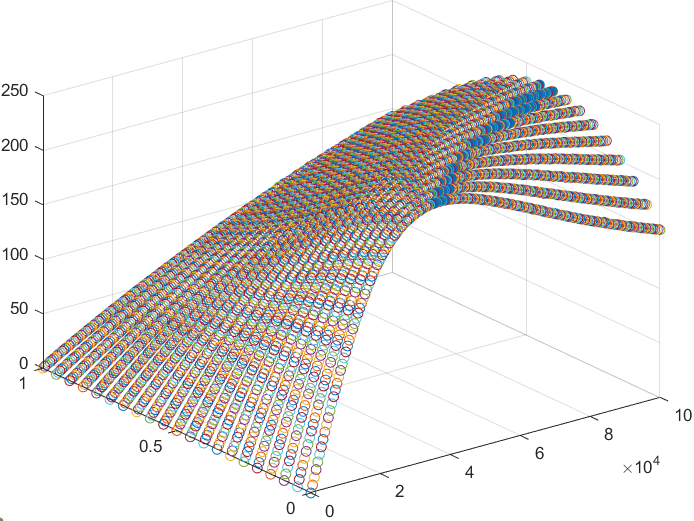
\includegraphics[scale=0.3]{问题2-2整体.png} \label{1}
    }
    \subfigure[最大值点在$\alpha-k_{\eta_p}$平面投影]{
    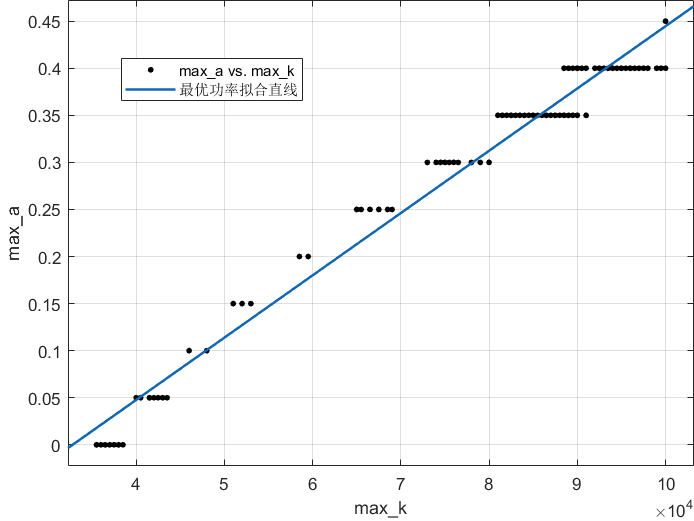
\includegraphics[scale=0.3]{问题2-2投影.png} \label{2} 
    }
    \quad
    \caption{问题2-2$\;\,p-k_{\eta _p},\alpha$散点图}
\end{figure}
检索遍历数据中平均功率最大的100个点,在图7(a)中用蓝色标出并投影到$\alpha-k_{\eta _p}$平面,得到图7(b)数据点。由检索数据可知(程序见附录B.1):100个最大值点对应的功率极差小于$0.5W$,不足平均值$234.4W$的四百分之一,各点处平均功率的差别可以忽略。但最大值数据点在图7(b)上分布较为分散,故使用直线拟合描述最大输出功率对应的$k_{\eta _p}$与$\alpha$,拟合函数$\alpha=6.616\times 10^{-6}k_{\eta_p}-0.2169$,拟合度$R^2=0.97$,拟合结果如图7(b)蓝线所示。

考虑x现实应用中其他因素对阻尼器的影响,实际最优点对应的$k_{\eta_p}$与$\alpha$可能较理想解稍有偏移。结合图7(a)数据散点的拱面形状,选择拟合直线的中点作为最大平均功率点,最大化减小误差与其他因素带来的影响。

\textbf{【结论】}最大平均功率$P_{max}=234.4644W$,对应的比例系数$k_{\eta_p}=66392$,幂指数$\alpha=0.2223$






{\centering\section{问题三模型的建立与求解}}

\subsection{模型建立}
已知直线阻尼器的阻尼系数$\eta _{p}=10000 N·s/m$,旋转阻尼器的阻尼系数$\eta_r=1000 N·m·s$.计算可得浮子重心位于转轴沿浮子中心轴向上$d=1.4m$的位置.设$x_{g0}=x_0+d$,则绕水平过重心的轴的转动惯量为$J_0=5231.83 kg·m^2$。又考虑初始状态下浮子圆锥部分未露出水面,由于运动的连续性,浮子在开始运动的一段时间内圆锥部分仍位于水面之下。在浮子开始运动至圆锥部分未出水的时段,选取任意时刻分析浮子与振子的运动状态。
\begin{equation}
\left\{\begin{array}{l}
   \text{浮子受到的浮力:}F_{21}=m_{x} g +m_{z} g+\rho g \pi r^{z}\left(x_{g0}-\frac{x_g}{cos(\beta)}\right)\\
   \text{浮子受到的重力:}F_{22}=-m_{x} g\\
   \text{浮子受到的波峰激励力:}F_{23}=f \cos \omega t\\
   \text{浮子受到的兴波阻尼力:}F_{24}=-\eta_{\text{兴}} \dot{x_g}\\
   \text{浮子受到的弹簧与阻尼器作用力:}F_{25}=\cos(\alpha)[-k\left(l_{0}-z_p\right)+\eta_{p}(\dot{z_p})]\\
\end{array}\right.
\end{equation}

根据牛顿第二定律,$F_{21}+F_{22}+F_{23}+F_{24}+F_{25}=(m_x+M)\ddot{x_g}$,整理得:
\begin{equation}
m_{z} g+\rho g \pi r^{z}\left(x_{0}-\frac{x_g}{cos(\beta)}\right)+f \cos \omega t-\eta_{\text{兴}} \dot{x_g}+\cos(\alpha)[-k\left(l_{0}-z_p\right)+\eta_{p}(\dot{z_p})]=\left(m_{x}+M\right) \ddot{x_g}
\end{equation}


考虑浮子绕重心所在轴旋转时所受到的力矩
\begin{equation}
    \left\{\begin{array}{l}
        \text{浮子受到的激励力矩:}M_{11}=L\cos(\omega t)\\
        \text{浮子受到的兴波阻尼力力矩:}M_{12}=-k_{兴}\dot{\beta}\\
        \text{浮子受到的静水恢复力矩:}M_{13}=-k_{恢}\beta\\
        \text{浮子受到的来自转轴处的力矩:}M_{14}=k_r\alpha+\eta_r\dot{\alpha}\\
    \end{array}\right.
    \end{equation}

由于$M_{11}+M_{12}+M_{13}+M_{14}=(J_0+J_f)\ddot{\beta}$,整理得:
\begin{equation}
    L\cos(\omega t)-k_{兴}\dot{\beta}-k_{恢}\beta+k_r\alpha+\eta_r\dot{\alpha}=(J_0+J_f)\ddot{\beta}
\end{equation}

考虑振子沿杆方向所受到的力
\begin{equation}
\left\{\begin{array}{l}
    \text{振子受到的重力:}F_{26}=-m_{z} g\cos(\alpha)\\
    \text{振子受到的弹簧与阻尼器作用力:}F_{27}=k\left(l_{0}-z_p\right)-\eta_{p}(\dot{z_p})\\
    \text{振子受到的惯性力:}F_{28}=-\cos(\alpha+\beta)\ddot{x_g}+\sin(\alpha)\ddot{\alpha}d\\
\end{array}\right.
\end{equation}

根据牛顿第二定律,$F_{26}+F_{27}+F_{28}=m_{z} \ddot{z_p}$,整理得:
\begin{equation}
    -m_{z} g\cos(\alpha)+k\left(l_{0}-z_p\right)-\eta_{p}(\dot{z_p})-\cos(\alpha+\beta)\ddot{x_g}+\sin(\alpha)\ddot{\alpha}d=m_{z} \ddot{z_p}
\end{equation}

考虑转轴处所受到的力矩,振子对于转轴的转动惯量为$J_z=m_zz_p^2$
\begin{equation}
    \left\{\begin{array}{l}
        \text{转轴受到的扭转弹簧扭矩}M_{15}=-k_r\alpha\\
        \text{转轴受到的旋转阻尼器的扭矩:}M_{16}=-\eta_r\dot{\alpha}\\
        \text{振子重力对转轴的力矩:}M_{17}=\sin{\alpha}m_zgz_p\\
        \text{振子惯性力对转轴的力矩:}M_{18}=J_z[-\sin(\alpha+\beta)\ddot{x_g}-cos(\alpha)\ddot{\alpha}d]\\
    \end{array}\right.
\end{equation}

由于$M_{15}+M_{16}+M_{17}+M_{18}=J_z\ddot{\alpha}$,整理得:
\begin{equation}
    -k_r\alpha-\eta_r\dot{\alpha}+\sin{\alpha}m_zgz_p-J_z[\sin(\alpha+\beta)\ddot{x_g}-cos(\alpha)\ddot{\alpha}d]=J_z\ddot{\alpha}
\end{equation}

整理方程(7.1.2),(7.1.4),(7.1.6),(7.1.8),换元$\dot{x_g}=v_{x_g},\dot{\beta}=v_{\beta},\dot{z_p}=v_{z_p},\dot{\alpha}=v_{\alpha} $,得一阶显式微分方程组:
\begin{equation}
\left\{\begin{array}{l}
    \dot{x_g}=v_{x_g}\;,\;\dot{\beta}=v_{\beta}\;,\;\dot{z_p}=v_{z_p}\;,\;\dot{\alpha}=v_{\alpha} \\
    m_{z} g+\rho g \pi r^{2}\left(x_{g0}-\frac{x_g}{cos(\beta)}\right)+f \cos \omega t-\eta_{\text{兴}}v_{x_g}+\cos(\alpha)[-k\left(l_{0}-z_p\right)+\eta_{p}(\dot{z_p})]=\left(m_{x}+M\right) \dot{v_{x_g}}\\
    L\cos(\omega t)-k_{兴}v_{\beta}-k_{恢}\beta+k_r\alpha+\eta_rv_{\alpha}=(J_0+J_f)\dot{v_\beta}\\
    -m_{z} g\cos(\alpha)+k\left(l_{0}-z_p\right)-\eta_{p}(v_{z_p})-\cos(\alpha+\beta)\dot{v_{x_g}}+\sin(\alpha)\dot{v_{\alpha}}d=m_{z} \dot{v_{z_p}}\\
    -k_r\alpha-\eta_rv_{\alpha}+\sin{\alpha}m_zgz_p-m_zz_p^2[\sin(\alpha+\beta)\dot{v_{x_g}}-cos(\alpha)\dot{v_{\beta}}d]=m_zz_p^2\dot{v_{\alpha}}\\
\end{array}\right.
\end{equation}


\subsection{模型求解}
调用 matlab 中的odefun函数求解方程组 (7.1.9) 的数值解 (程序见附录 C)。以 0.2s 为步
长得到各时刻浮子与振子的垂荡位移、垂荡速度、纵摇偏移角、纵摇角速度,整理数据并绘制散点图。详见附录C。


在建模过程中,我们仅描述了浮子开始运动至圆锥部分未出水时段中任意时刻的运动状态。由推得的浮子位置与时间关系可知,此阶段运动中浮子圆锥部分并未露出水面。由运动的连续性可以推得,浮子垂荡运动全程圆锥部分均不会露出水面,模型求解得到的结论数据即为浮子与振子的全程运动数据。将得到的数据存储于result3.xlsx文件中,提取10s、20s、40s、60s、100时刻数据如下表:


\begin{figure}[H]
    \centering
    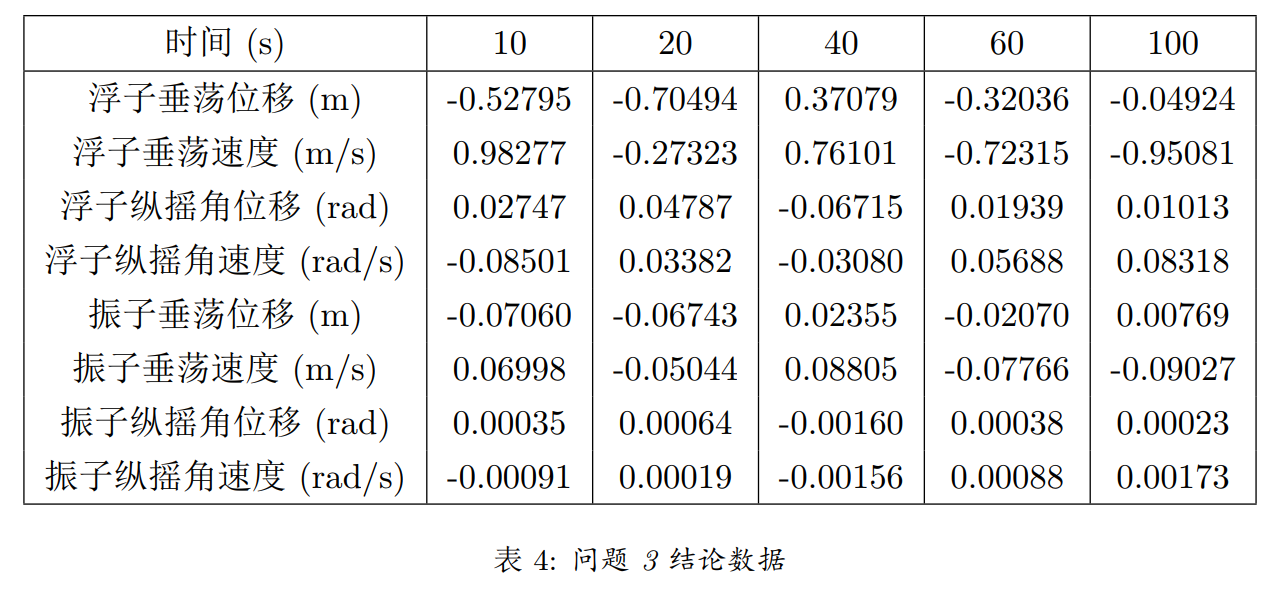
\includegraphics[scale=0.5]{问题3结论表.png}
\end{figure}


\newpage


%\begin{table}[!htbp]
%   \centering
%    \begin{tabular}{|c|c|c|c|c|c|}\hline
%        时间 (s)&	10	&	20	&	40&		60	&	100\\\hline
%浮子垂荡位移 (m)	&	-0.52795 &		-0.70494 &		0.37079 &		-0.32036 	&	-0.04924 \\
%浮子垂荡速度 (m/s)	&	0.98277 &		-0.27323 &		0.76101 	&	-0.72315 	&	-0.95081 \\
%浮子纵摇角位移(rad) &		0.02747 &		0.04787 &		-0.06715 &		0.01939 &		0.01013 \\
%浮子纵摇角速度 (rad/s)&		-0.08501 &		0.03382 &		-0.03080 &		0.05688 &		0.08318 \\
%振子垂荡位移 (m)	&	-0.07060 &		-0.06743 &		0.02355 	&	-0.02070 &		0.00769 \\
%振子垂荡速度 (m/s)&		0.06998 	&	-0.05044 &		0.08805 &		-0.07766 &		-0.09027 \\
%振子纵摇角位移(rad)	&	0.00035 &		0.00064 	&	-0.00160 &		0.00038 &		0.00023 \\
%振子纵摇角速度 (rad/s)&		-0.00091 	&	0.00019 &		-0.00156 &		0.00088 &		0.00173 \\

 %       \hline
 %  \end{tabular}
%    \caption{问题3结论数据}
%\end{table}
%表格具体尺寸参数调整:https://blog.csdn.net/u010158659/article/details/78964030




{\centering\section{问题四模型的建立与求解}}

\subsection{模型建立}
推导PTO系统平均功率表达式可得:
\begin{equation}
P=\frac{\Delta W}{\Delta t}=\frac{\Delta W_{p\text {阻尼 }}+\Delta W_{r\text {阻尼}}}{\Delta t}=\frac{1}{\Delta t}\left(\int_{t_0}^{t_1} F_{\text{阻尼}} d z+\int_{t_0}^{t_1} M_{\text{阻尼}} d \alpha \right)
\end{equation}

其中$\Delta W_{p\text {阻尼 }}$、$ F_{\text{阻尼}}$分别表示直线阻尼器做功及其阻力,$\Delta W_{r\text {阻尼}}$、$M_{\text{阻尼}}$分别表示旋转阻尼器做功及其阻力矩。其中$F_{\text{阻尼}}=\eta _p v_{zp},M_{\text{阻尼}}=\eta _r v_{\alpha}$,代入表达式(8.1.1)可得:
\begin{equation}
P=\frac{1}{\Delta t}\left(\eta_{p} \int_{t_{0}}^{t_{1}} v_{zp}^{2} d t+\eta_{r} \int_{t_{0}}^{t_{1}} v_{\alpha}^{2} d t\right)    =   \frac{1}{\Delta t} \int_{t_{0}}^{t_{1}}\left(\eta_{p} v_{zp}^{2}+\eta_{r} v_{\alpha}^{2}\right) d t
\end{equation}

使用数值积分的梯形积分法求解平均功率,取$t_0=20 \times \frac{2 \pi}{\omega}, \; t_{1}=40 \times \frac{2 \pi}{\omega}\Delta t=t_1-t_0$
\begin{equation}
P=\frac{1}{\Delta t}\sum\limits_{i=1}^{n-1}\frac{\Delta v(i+1)^2+\Delta v(i)^2}{2}h
\end{equation}

其中$\eta_p v_{zp}^2+\eta_r v_{\alpha}^2=\Delta v^2,\;h=0.2s$
\subsection{模型求解}


已知平均最大功率是关于直线阻尼系数$\eta _p$与旋转阻尼系数$\eta _r$的函数。定义域$\eta_p \in [0,100000]$,$\;\eta _r\in [0,100000]$,可视为一个较大的$100000\times 100000$正方形区域。由于直接进行高密度搜索需要的时间成本较高,这里采用多重搜索方法求解最大平均功率点。

首先对区间$[0,100000]$以500为步长做遍历,得到不同的阻尼系数对应的平均功率数据并绘制散点图如图8(a)。检索其最大值点在$\eta_p-\eta_r$平面投影的位置,继而以该点为中心,在$1000\times1000$的正方形区域内以50为步长进行遍历……如此循环,对于$\eta_p-\eta_r$平面上一块$n\times n$的区域,以步长为$\frac{n}{20}$进行遍历,再在平均功率最大值点为中心$\frac{n}{10}$为边长的区域内以$\frac{n}{200}$为步长进行遍历,最终将遍历区域边长缩小至$10$,绘制数据散点图如下:

%\begin{figure}[H]
%    \centering
%    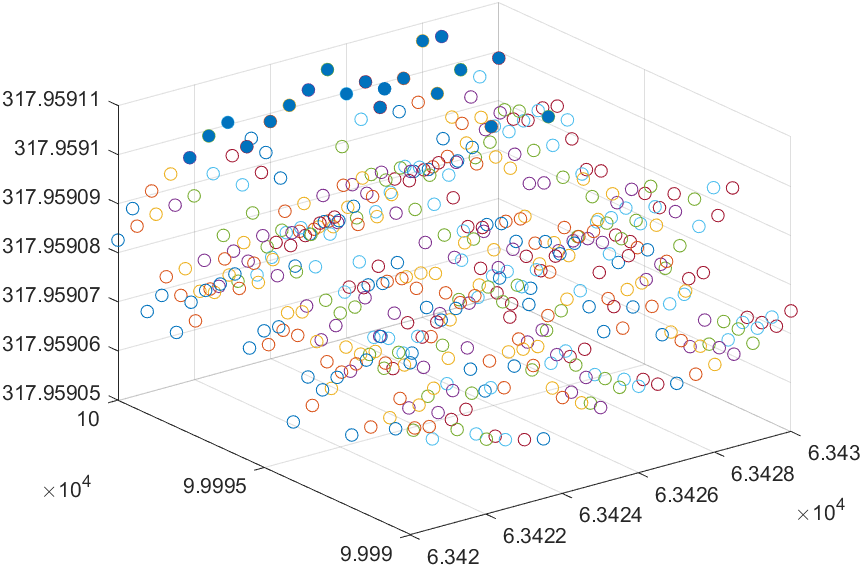
\includegraphics[scale=0.75]{问题4散点图.png}
%    \caption{问题4局部数据散点图}
%\end{figure}
\begin{figure}[htbp]
    \centering
    \subfigure[首次遍历数据散点图]{
    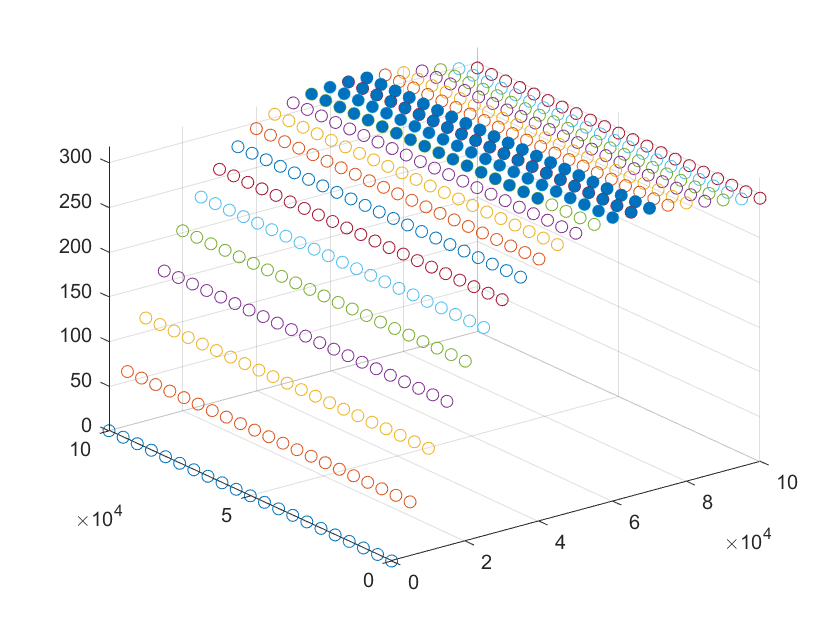
\includegraphics[scale=0.3]{问题4原始图.png} \label{1}
    }
    \subfigure[末次遍历数据散点图]{
    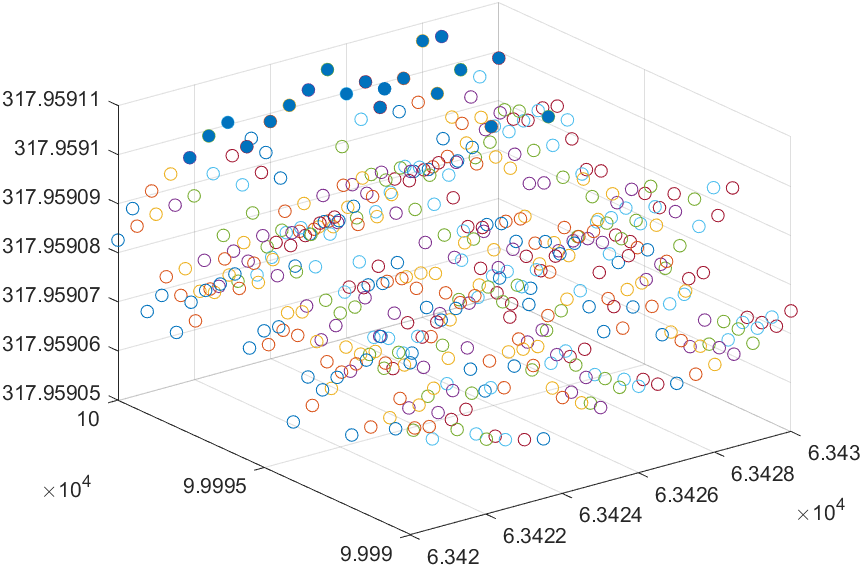
\includegraphics[scale=0.5]{问题4散点图.png} \label{2} 
    }
    \quad
    \caption{问题4遍历数据散点图}
\end{figure}
此时正方形遍历区间边长为定义域长度的万分之一,多重搜索已经达到了较高精度,可取范围内平均功率最大值点作为结论数据。

\textbf{【结论】}最大平均输出功率$P_{max}=317.9591W$,相应的阻尼系数$\eta_p=63428N·s/m,\eta _r=100000N·s·m$


{\centering\section{模型的评价与改进}}
\subsection{模型的优点}
1.在问题一和问题三中,我们通过建立完整、细致的微分方程组,并将其转化为一阶显式微分方程组,使得题目可解且理论上精确。利用Matlab中的ode45微分方程数值求解器求解,增大了求解的精度,使得到数据更接近实际。

2.在问题二和问题四中,我们对功率的计算采取数学推导与数值分析结合的方式。通过对数据的观察,提炼出数据稳定的区间,并在一段时间上对做功进行平均,得到平均功率。对于做功,我们利用梯形对积分的近似,使得理论推导与数值演算更加快速且精准。为最大值的搜索简化了模型,提高了计算速度。

3.我们采用隔离法和整体法两种思路进行建模,对比后发现隔离法建模更贴近实际。
\subsection{模型的缺点}
1.在问题三和问题四的情境下,由于转动惯量与力矩数值上量级的差距,导致建模所求得的角位移和角速度偏小,影响整体求解。

2.对问题三、问题四的情境过于简化。为了建模的简便,我们假设了浮子旋转轴位于重心处,并且转轴相对浮子位置不改变。实际上和真实情况相差甚远,真实情况的稳心要高于重心,导致计算求解过程中关于角度的计算不够精确。

3.对于最大功率的搜索,通过遍历、多重搜索进行查找,计算量过于大,程序耗时长。
\subsection{模型的改进与推广}
1.对于问题二与问题四中最大值的搜索,可以再考虑利用蒙德卡洛方法或者遗传算法进行寻找,降低耗时。

2.对于问题三、问题四的情境,引入有关稳心、浮心的相关物理量,对于各个力的作用点进行详尽的分析,确定更加准确的浮子、振子转动力矩,从而得到更加精确和真实的角位移与角速度。

3.尝试利用物理软件进行仿真,通过各个时间节点仿真结果,通过相关系数来评价模型的准确程度。

4.本题仅涉及了浮子两个自由度的运动,将其推广至实际问题。实际问题中需要考虑6个自由度的运动,以及浮子内振子的多自由度运动,可以尝试通过矩阵与复数的方式进行微分方程组建模,求得精值。









{\centering\section{参考文献}}
\begingroup  % 去掉thebibliography环境自带的“参考文献”标题
\renewcommand{\section}[2]{}
\begin{thebibliography}{99}
    
\bibitem{1}
谢惠媚,孟凡泰,徐潜龙. 不同形状的多自由度内置PTO式波浪能转换装置的性能分析[J] . 可再生能源 . 2022.7 .第40卷第7期. 986-994

\bibitem{2}
高 琅,朱良生,王 磊,周斌珍. 垂荡式波浪能装置与风机平台集成系统水动力性能研究[J] . 广东造船 . 2022.3 .2022年第3期(总第184)期. 17-21

\bibitem{3}
Timonthy Sauer. Numerical Analysis[M] . 北京 . 机械工业出版社 . 2014 . 226-227

\bibitem{4}
国威. 震荡浮子式波浪能装置水动力特性CFD数值模拟[D] . 哈尔滨 . 哈尔滨工程大学 . 2016



%\bibitem{最小二乘}
%胡耀垓,张晓星,赵正予,冯 波. 光谱重叠峰的曲线拟合解析策略与实现[J] . 信息系统工程 . 2012.5 .第35卷第5期. 76-82

%\bibitem{最小二乘}
%胡耀垓,张晓星,赵正予,冯 波. 光谱重叠峰的曲线拟合解析策略与实现[J] . 信息系统工程 . 2012.5 .第35卷第5期. 76-82

\end{thebibliography}
\endgroup

\newpage



{\centering\section*{附录}}
\appendix
\section{问题一相关数据及代码}

\subsection{问题1-1微分方程数值解求解及绘图代码}
构造\verb|odefun|函数
\begin{lstlisting}
    function dxz=odefun(t,xz)
    V=(4866+2433)/1025; 
    V1=1/3*pi*0.8; 
    x0=-(V-V1)/pi;
    z0=x0+0.5-2433*9.8/80000;
    ro=1025;g=9.8;M=1335.535;w=1.4005;etax=656.3616;etap=10000;L0=0.5;mx=4866;mz=2433;r=1;f=6250;k=80000;
    %%二维的变量,xz(1)=x,xz(2)=z,xz(3)=vx,xz(4)=vz 
    dxz=zeros(4,1); 
    dxz(1)=xz(3); 
    dxz(2)=xz(4);
    dxz(3)=(mz*g+ro*g*pi*r*r*(x0-xz(1))+f*cos(w*t)-etax*xz(3)-k*(L0-xz(2)+xz(1))-etap*(xz(3)-xz(4)))/(mx+M) ;
    dxz(4)=(k*(L0-xz(2)+xz(1))+etap*(xz(3)-xz(4))-mz*g)/mz; 
    end
\end{lstlisting}

微分方程求解及绘图
\begin{lstlisting}
    clear
    clc
    format long
    V=(4866+2433)/1025;
    V1=1/3*pi*0.8;
    x0=-(V-V1)/pi;
    z0=x0+0.5-2433*9.8/80000;
    x1=0;z1=0;
    [t,xz]=ode45('odefun',[0:0.02:40*2*pi/1.4005],[x0;z0;x1;z1]);       %作图
    [t1,xz1]=ode45('odefun',[0:0.2:40*2*pi/1.4005],[x0;z0;x1;z1]);      %excel
    [t2,xz2]=ode45('odefun',[0:10:120],[x0;z0;x1;z1]);      %论文
    plot(t,xz(:,1),'-',t,xz(:,2),'-')%浮子与振子位置
    %plot(t,xz(:,3),'-',t,xz(:,4),'-')%浮子与振子速度
    xfu=xz1(:,1)-x0;
    zzhen=xz1(:,2)-z0;
    vxfu=xz1(:,3);
    vzhen=xz1(:,4);
    
\end{lstlisting}


\subsection{问题1-1微分方程数值解求解及绘图代码}
构造\verb|odefun|函数
\begin{lstlisting}
    function dxz=odefun2(t,xz)
    V=(4866+2433)/1025; 
    V1=1/3*pi*0.8; 
    x0=-(V-V1)/pi;
    z0=x0+0.5-2433*9.8/80000;
    ro=1025;g=9.8;M=1335.535;w=1.4005;etax=656.3616;knp=10000;L0=0.5;mx=4866;mz=2433;r=1;f=6250;k=80000;
    %%二维的变量,xz(1)=x,xz(2)=z,xz(3)=vx,xz(4)=vz 
    dxz=zeros(4,1); 
    dxz(1)=xz(3); 
    dxz(2)=xz(4);
    dxz(3)=(mz*g+ro*g*pi*r*r*(x0-xz(1))+f*cos(w*t)-etax*xz(3)-k*(L0-xz(2)+xz(1))-knp*abs(xz(3)-xz(4)).^0.5*(xz(3)-xz(4)))/(mx+M) ;
    dxz(4)=(k*(L0-xz(2)+xz(1))+knp*abs(xz(3)-xz(4)).^0.5*(xz(3)-xz(4))-mz*g)/mz; 
    end
\end{lstlisting}

微分方程求解及绘图
\begin{lstlisting}
    clear
    clc
    format long
    V=(4866+2433)/1025;
    V1=1/3*pi*0.8;
    x0=-(V-V1)/pi;
    z0=x0+0.5-2433*9.8/80000;
    x1=0;z1=0;
    [t,xz]=ode45('odefun2',[0:0.02:40*2*pi/1.4005],[x0;z0;x1;z1]);   %作图
    [t1,xz1]=ode45('odefun2',[0:0.2:40*2*pi/1.4005],[x0;z0;x1;z1]);     %excel
    [t2,xz2]=ode45('odefun2',[0:10:120],[x0;z0;x1;z1]);  %论文
    plot(t,xz(:,1),'-',t,xz(:,2),'-')%浮子与振子位置
    %plot(t,xz(:,3),'-',t,xz(:,4),'-')%浮子与振子速度
    
    xfu=xz1(:,1)-x0;
    zzhen=xz1(:,2)-z0;
    vxfu=xz1(:,3);
    vzhen=xz1(:,4);
    
\end{lstlisting}

        



\section{问题二相关数据及代码}
\subsection{问题2-1绘图与检索估计代码}
\begin{lstlisting}
    etaps=[1:10:100000];
    p=zeros(1,10000);
    for i = 1:10000
    p(i)=powerp(etaps(i));
    end
    plot(etaps,p,'o-','MarkerSize',3)
    hold on
    [b,i]=sort(p);
    plot(etaps(i(end-9:end)),b(end-9:end),'*','MarkerSize',15)
    max=sum(b(end-9:end))/10;
    index=sum(etaps(i(end-9:end)))/10;

    function dxz=odefunqq(t,xz,etap)
    V=(4866+2433)/1025; 
    V1=1/3*pi*0.8; 
    x0=-(V-V1)/pi;
    z0=x0+0.5-2433*9.8/80000;
    ro=1025;g=9.8;M=1165.992;w=2.2143;etax=167.8395;L0=0.5;mx=4866;mz=2433;r=1;f=4890;k=80000;
    %%二维的变量,xz(1)=x,xz(2)=z,xz(3)=vx,xz(4)=vz 
    dxz=zeros(4,1); 
    dxz(1)=xz(3); 
    dxz(2)=xz(4);
    dxz(3)=(mz*g+ro*g*pi*r*r*(x0-xz(1))+f*cos(w*t)-etax*xz(3)-k*(L0-xz(2)+xz(1))-etap*(xz(3)-xz(4)))/(mx+M) ;
    dxz(4)=(k*(L0-xz(2)+xz(1))+etap*(xz(3)-xz(4))-mz*g)/mz; 
    end

    function p=powerp(etapx)
    V=(4866+2433)/1025;
    V1=1/3*pi*0.8;
    x0=-(V-V1)/pi;
    z0=x0+0.5-2433*9.8/80000;
    x1=0;z1=0;
    etap=etapx;
    [~,xz1]=ode45(@(t,xz1)odefunqq(t,xz1,etap),[0:0.2:40*2*pi/2.2143],[x0;z0;x1;z1]);
    vxfu=xz1(:,3);
    vzhen=xz1(:,4);
    square=(vxfu(fix(20*2*pi/2.2143)*5:fix(40*2*pi/2.2143)*5)-vzhen(fix(20*2*pi/2.2143)*5:fix(40*2*pi/2.2143)*5)).^2; %%取第20至第40个周期稳定后的值来计算平均做功
    area=1:(-fix(20*2*pi/2.2143)+fix(40*2*pi/2.2143))*5;
    for i=1:-fix(20*2*pi/2.2143)*5+fix(40*2*pi/2.2143)*5
    area(1,i)=(square(i,1)+square(i+1,1))*0.5*0.2;
    end
    p=etap*sum(area)/(20*2*pi/2.2143);
    end
\end{lstlisting}

\subsection{问题2-2绘图与检索估计代码}
最大值点检索与绘图
\begin{lstlisting}
    knps=[0:500:100000];
    alpha=[0:0.05:1];
    plist=zeros(201,21);%plist_k=zeros(201,21);plist_a=zeros(201,21);
    figure(1);
    for j=1:21
        for i = 1:201
        p=powerp2(knps(i),alpha(j));
        plist(i,j)=p;
        %plist_k(i,j)=i;plist_a(i,j)=j;
        scatter3(knps(i),alpha(j),p)
    hold on
        end
    end
    [B,IX] = sort(plist(:),'descend');
    [I,J] = ind2sub(size(plist),IX) ;
    scatter3(knps(I(1:80)),alpha(J(1:80)),B(1:80),'filled')
    max_k=knps(I(1:80));max_a=alpha(J(1:80));
    hold off 
    figure(2);
    figure2=scatter(knps(I(1:80)),alpha(J(1:80)),'filled');%最大80个点在alpha和阻尼系数平面上的投影
    
    % [m,im]=max(plist);
    % [m2,im2]=max(m);
    % i=im(im2);
    % j=im2;
    % k_index=knps(i);a_index=alpha(j);
    
    % plot(knp,p,'o-','MarkerSize',3)
    % hold on
    % [b,i]=sort(p);
    % plot(knp(i(end-9:end)),b(end-9:end),'*','MarkerSize',15)
    % max=sum(b(end-9:end))/10;
    % index=sum(knp(i(end-9:end)))/10;
       
    function dxz=odefunqq2(t,xz,knp,alpha)
    V=(4866+2433)/1025; 
    V1=1/3*pi*0.8; 
    x0=-(V-V1)/pi;
    z0=x0+0.5-2433*9.8/80000;
    ro=1025;g=9.8;M=1165.992;w=2.2143;etax=167.8395;L0=0.5;mx=4866;mz=2433;r=1;f=4890;k=80000;
    %%二维的变量,xz(1)=x,xz(2)=z,xz(3)=vx,xz(4)=vz 
    dxz=zeros(4,1); 
    dxz(1)=xz(3); 
    dxz(2)=xz(4);
    dxz(3)=(mz*g+ro*g*pi*r*r*(x0-xz(1))+f*cos(w*t)-etax*xz(3)-k*(L0-xz(2)+xz(1))-knp*abs(xz(3)-xz(4)).^alpha*(xz(3)-xz(4)))/(mx+M) ;
    dxz(4)=(k*(L0-xz(2)+xz(1))+knp*abs(xz(3)-xz(4)).^alpha*(xz(3)-xz(4)))/mz; 
    end
    
    function p=powerp2(knpx,alpha)
    V=(4866+2433)/1025;
    V1=1/3*pi*0.8;
    x0=-(V-V1)/pi;
    z0=x0+0.5-2433*9.8/80000;
    x1=0;z1=0;
    knp=knpx;
    [~,xz1]=ode45(@(t,xz1)odefunqq2(t,xz1,knp,alpha),[0:0.2:40*2*pi/2.2143],[x0;z0;x1;z1]);
    vxfu=xz1(:,3);
    vzhen=xz1(:,4);
    fix1=fix(20*2*pi/2.2143);fix2=fix(40*2*pi/2.2143);
    square=abs(vxfu(fix1*5:fix2*5)-vzhen(fix1*5:fix2*5)).^(alpha+2); %%取20-40个周期稳定后的值来计算平均做功
    area=1:(-fix1+fix2)*5;
    for i=1:-fix1*5+fix2*5
    area(1,i)=(square(i,1)+square(i+1,1))*0.1;
    end
    p=knp*sum(area)/(20*2*pi/2.2143);
    end
    
\end{lstlisting}
结果求解
\begin{lstlisting}
    p2 =  -0.2169;
    p1 =  6.616e-06;
    x0=-p2/p1;
    knp_best=(x0+100000)/2;
    alpha_best=knp_best*p1+p2;
    
    p_best=powerp2(knp_best,alpha_best);
    
    function dxz=odefunqq2(t,xz,knp,alpha)
    V=(4866+2433)/1025; 
    V1=1/3*pi*0.8; 
    x0=-(V-V1)/pi;
    z0=x0+0.5-2433*9.8/80000;
    ro=1025;g=9.8;M=1165.992;w=2.2143;etax=167.8395;L0=0.5;mx=4866;mz=2433;r=1;f=4890;k=80000;
    %%二维的变量,xz(1)=x,xz(2)=z,xz(3)=vx,xz(4)=vz 
    dxz=zeros(4,1); 
    dxz(1)=xz(3); 
    dxz(2)=xz(4);
    dxz(3)=(mz*g+ro*g*pi*r*r*(x0-xz(1))+f*cos(w*t)-etax*xz(3)-k*(L0-xz(2)+xz(1))-knp*abs(xz(3)-xz(4)).^alpha*(xz(3)-xz(4)))/(mx+M) ;
    dxz(4)=(k*(L0-xz(2)+xz(1))+knp*abs(xz(3)-xz(4)).^alpha*(xz(3)-xz(4)))/mz; 
    end
    
    function p=powerp2(knpx,alpha)
    V=(4866+2433)/1025;
    V1=1/3*pi*0.8;
    x0=-(V-V1)/pi;
    z0=x0+0.5-2433*9.8/80000;
    x1=0;z1=0;
    knp=knpx;
    [~,xz1]=ode45(@(t,xz1)odefunqq2(t,xz1,knp,alpha),[0:0.2:40*2*pi/2.2143],[x0;z0;x1;z1]);
    vxfu=xz1(:,3);
    vzhen=xz1(:,4);
    fix1=fix(20*2*pi/2.2143);fix2=fix(40*2*pi/2.2143);
    square=abs(vxfu(fix1*5:fix2*5)-vzhen(fix1*5:fix2*5)).^(alpha+2); %%取20-40个周期稳定后的值来计算平均做功
    area=1:(-fix1+fix2)*5;
    for i=1:-fix1*5+fix2*5
    area(1,i)=(square(i,1)+square(i+1,1))*0.1;
    end
    p=knp*sum(area)/(20*2*pi/2.2143);
    end
    
\end{lstlisting}


\section{问题三相关数据及代码}

构建\verb|oddfun|函数
\begin{lstlisting}
    function dxb=odefun_q3_1(t,xb)%隔离法
    V=(4866+2433)/1025; 
    V1=1/3*pi*0.8; 
    x0=-(V-V1)/pi+1.4;
    z0=0.5-2433*9.8/80000;
    mx=4866;r=1;mz=2433;ro=1025;g=9.8;k=80000;l0=0.5;kr=250000;kh=8890.7;
    w=1.7152;M=1028.876;Jf=7001.914;etax=683.4558;kx=654.3383;f=3640;L=1690;
    etap=10000;etar=1000;J0=5231.83;
    dxb=zeros(8,1);
    %xb(1)=x;xb(2)=beta;xb(3)=z;xb(4)=alpha;xb(5)=vx;xb(6)=vbeta;xb(7)=vz;xb(8)=valpha;
    dxb(1)=xb(5);
    dxb(2)=xb(6);
    dxb(3)=xb(7);
    dxb(4)=xb(8);
    dxb(5)=(mz*g+ro*g*pi*r^2*(x0-xb(1)/cos(xb(2)))+f*cos(w*t)-etax*xb(5)+etap*xb(7)*cos(xb(2)+xb(4))-k*(l0-xb(3))*cos(xb(4)+xb(2)))./(mx+M);
    dxb(6)=(L*cos(w*t)-kx*xb(6)-kh*xb(2)+kr*xb(4)+etar*xb(8))./(J0+Jf);
    dxb(7)=(k*(l0-xb(3))-etap*xb(7)-cos(xb(4)+xb(2))*mz*g)./mz-cos(xb(4)+xb(2))*dxb(5)+sin(xb(4))*1.4*dxb(6);
    dxb(8)=(-kr*xb(4)-etar*xb(8)+sin(xb(4)+xb(2))*mz*g*xb(3))./(mz*xb(3)*xb(3))-sin(xb(4)+xb(2))*dxb(5)-cos(xb(4))*1.4*dxb(6);
    end
\end{lstlisting}
微分方程求解及绘图
\begin{lstlisting}
    format long
    %隔离法
    V=(4866+2433)/1025; 
    V1=1/3*pi*0.8; 
    x0=-(V-V1)/pi+1.4;
    z0=0.5-2433*9.8/80000;
    b0=0;a0=0;
    w=1.7152;
    x1=0;z1=0;b1=0;a1=0;
    [t,xb]=ode45(@(t,xb)odefun_q3_1(t,xb),[0:0.02:40*2*pi/w],[x0,b0,z0,a0,x1,b1,z1,a1]);%作图数据来源
    [t1,xb1]=ode45(@(t,xb)odefun_q3_1(t,xb),[0:0.2:40*2*pi/w],[x0,b0,z0,a0,x1,b1,z1,a1]);%result3数据来源
    [t2,xb2]=ode45(@(t,xb)odefun_q3_1(t,xb),[0:10:40*2*pi/w],[x0,b0,z0,a0,x1,b1,z1,a1]);%论文需要(间隔10s)数据来源
    %xb(1)=x;xb(2)=beta;xb(3)=z;xb(4)=alpha;xb(5)=vx;xb(6)=vbeta;xb(7)=vz;xb(8)=valpha;
    xb1(:,1)=xb1(:,1)-x0;
    xb1(:,3)=xb1(:,3)-z0;
    xb2(:,1)=xb2(:,1)-x0;
    xb2(:,3)=xb2(:,3)-z0;

    plot(t,xb(:,1)-x0,'g')%x浮子垂荡位移
    title('浮子垂荡位移随时间变化关系图')
    plot(t,xb(:,2),'r')%beta浮子的纵摇偏移角
    title('浮子的纵摇偏移角随时间变化关系图')
    plot(t,xb(:,3)-z0,'b')%z振子垂荡位移
    title('振子垂荡位移随时间变化关系图')
    plot(t,xb(:,4),'k')%alphaz振子纵摇偏移角
    title('振子纵摇偏移角随时间变化关系图')
    plot(t,xb(:,5),'g')%浮子垂荡速度
    title('浮子垂荡速度随时间变化关系图')
    plot(t,xb(:,6),'r')%浮子纵摇角速度
    title('浮子纵摇角速度随时间变化关系图')
    plot(t,xb(:,7),'b')%振子垂荡速度
    title('振子垂荡速度随时间变化关系图')
    plot(t,xb(:,8),'k')%振子纵摇角速度
    title('振子纵摇角速度随时间变化关系图')
\end{lstlisting}

所求物理量随时间变化关系图
\begin{figure}[H]
    \centering
    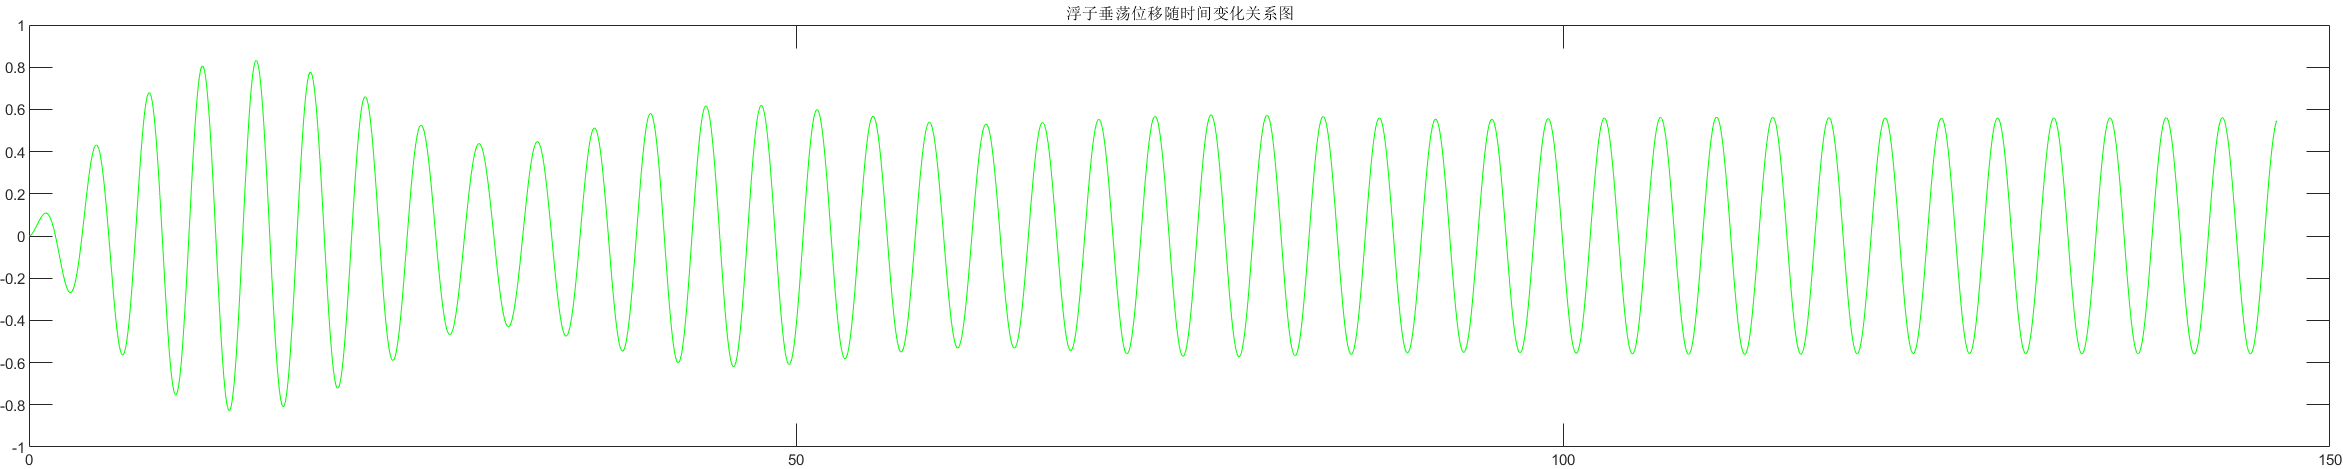
\includegraphics[scale=0.3]{问题3-1.png}
    \caption{浮子垂荡位移随时间变化关系图}
\end{figure}
\begin{figure}[H]
    \centering
    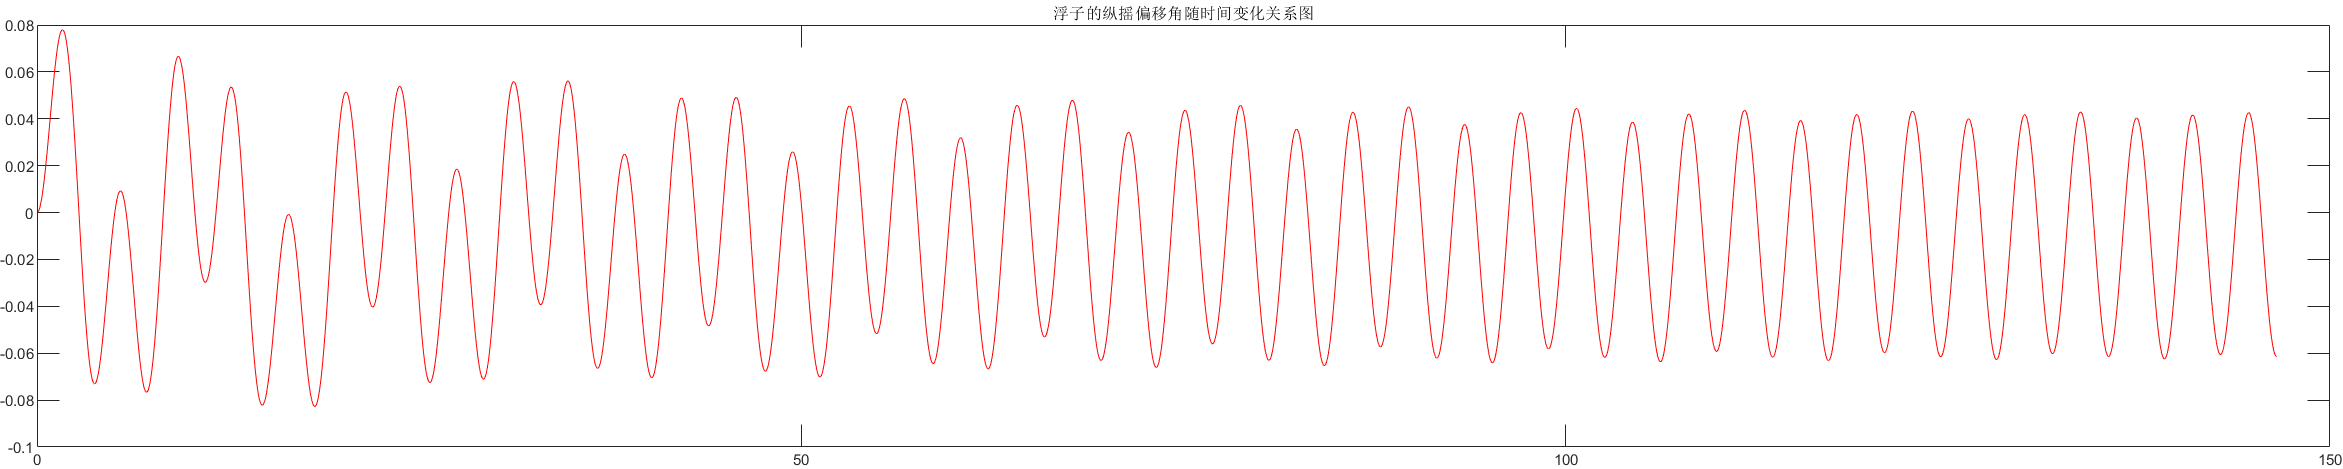
\includegraphics[scale=0.3]{问题3-2.png}
    \caption{浮子的纵摇偏移角随时间变化关系图}
\end{figure}
\begin{figure}[H]
    \centering
    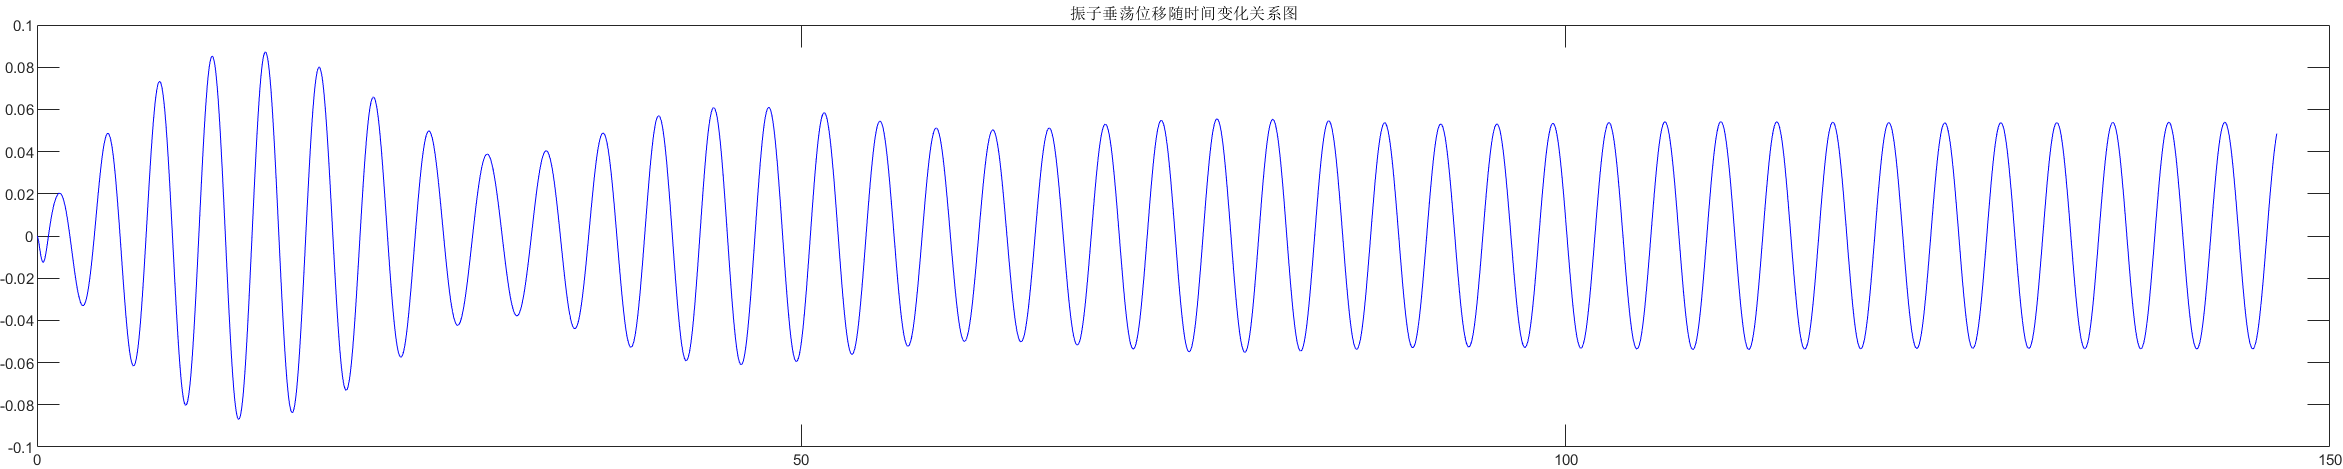
\includegraphics[scale=0.3]{问题3-3.png}
    \caption{振子垂荡位移随时间变化关系图}
\end{figure}
\begin{figure}[H]
    \centering
    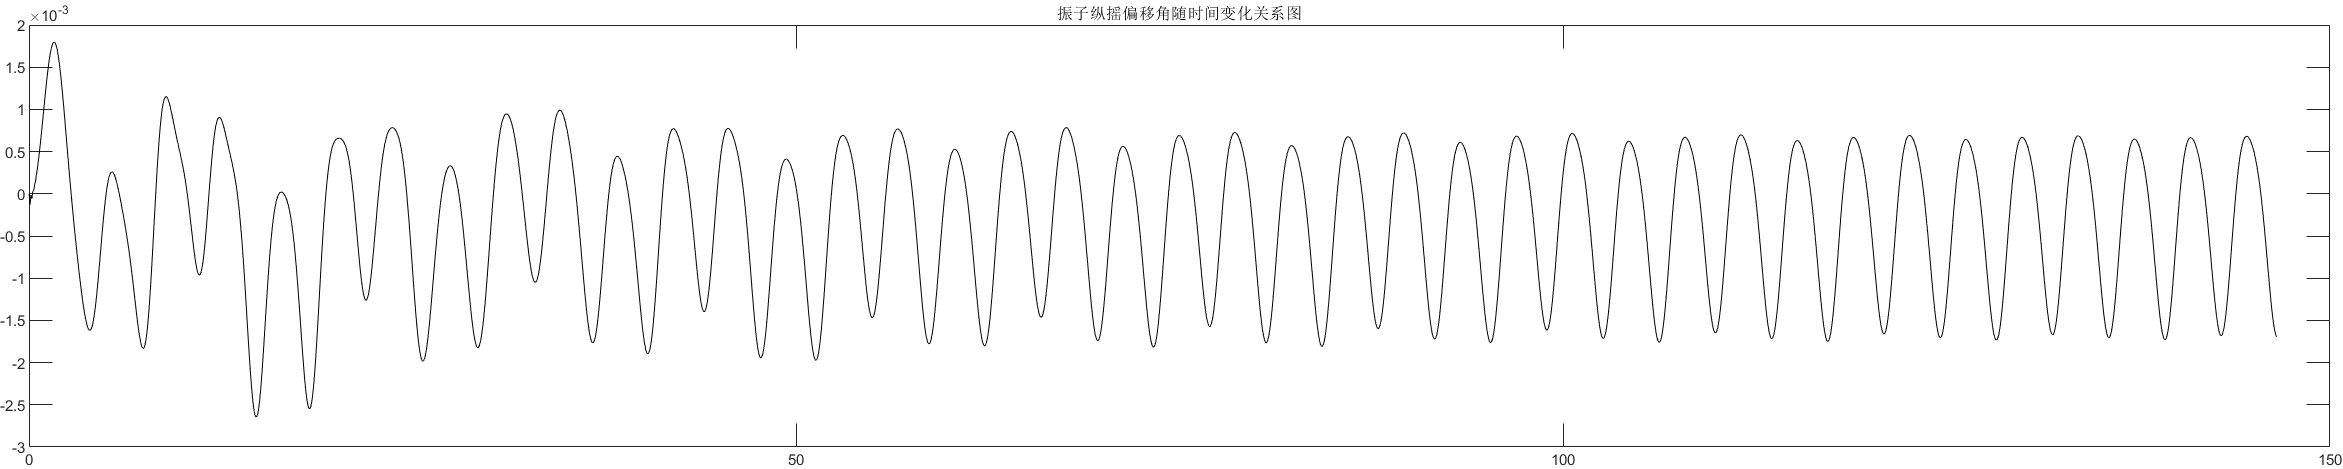
\includegraphics[scale=0.3]{问题3-4.png}
    \caption{振子纵摇偏移角随时间变化关系图}
\end{figure}
\begin{figure}[H]
    \centering
    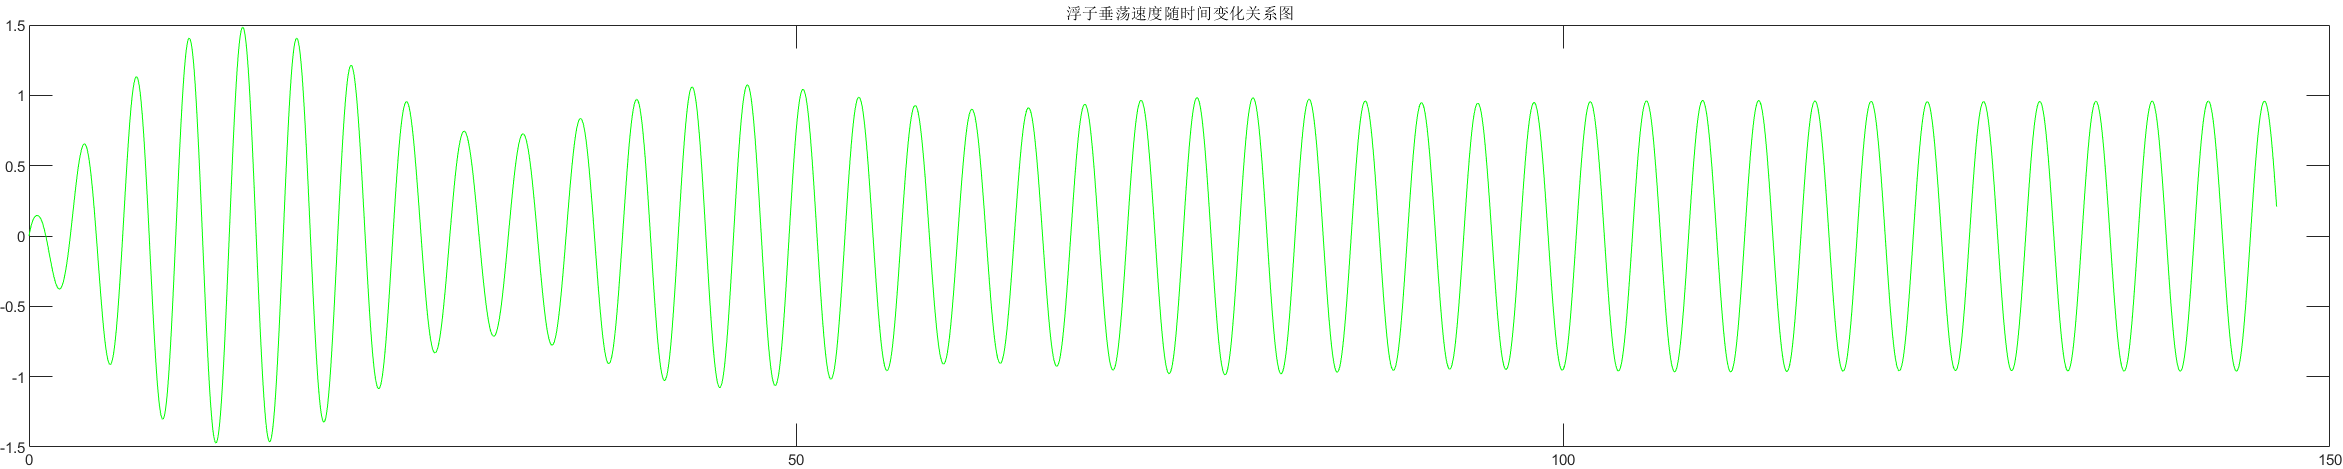
\includegraphics[scale=0.3]{问题3-5.png}
    \caption{浮子垂荡速度随时间变化关系图}
\end{figure}
\begin{figure}[H]
    \centering
    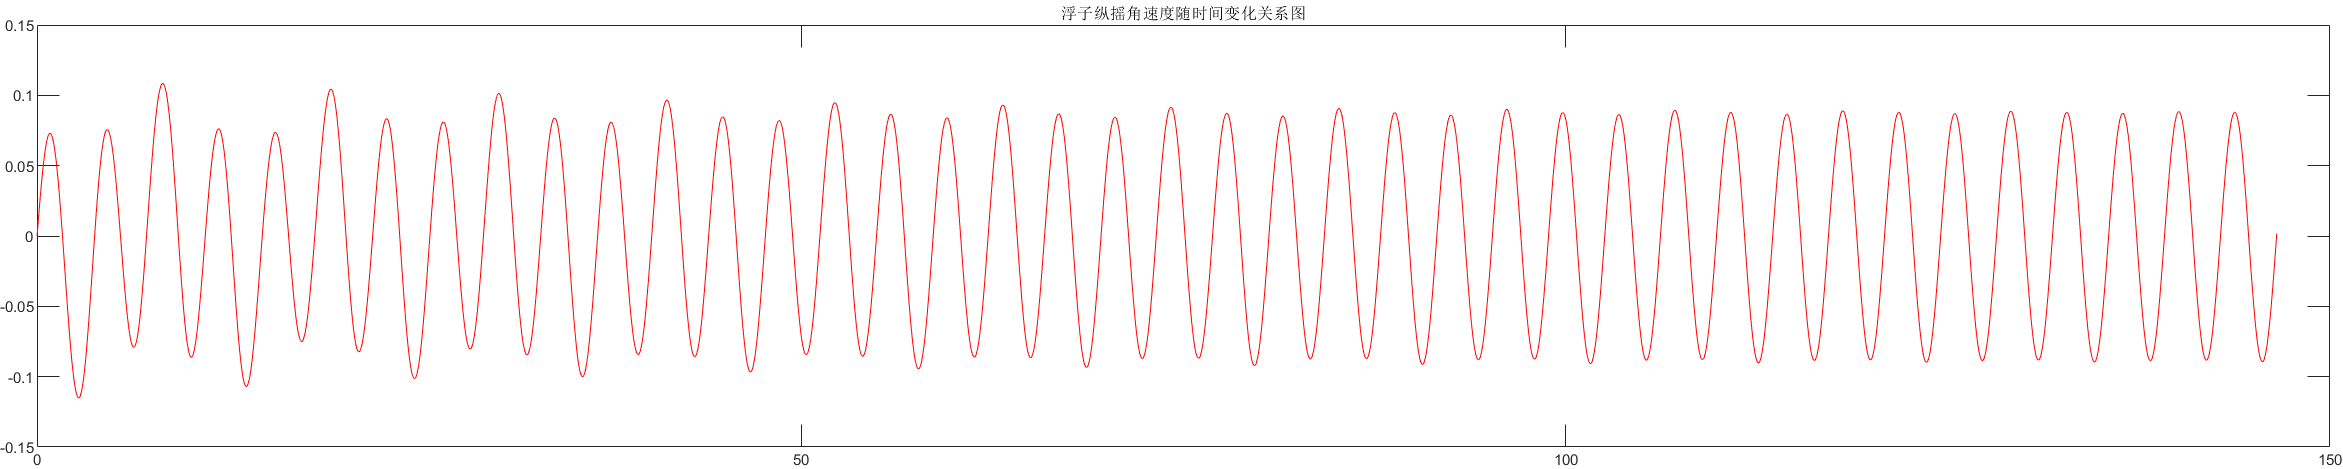
\includegraphics[scale=0.3]{问题3-6.png}
    \caption{浮子纵摇角速度随时间变化关系图}
\end{figure}
\begin{figure}[H]
    \centering
    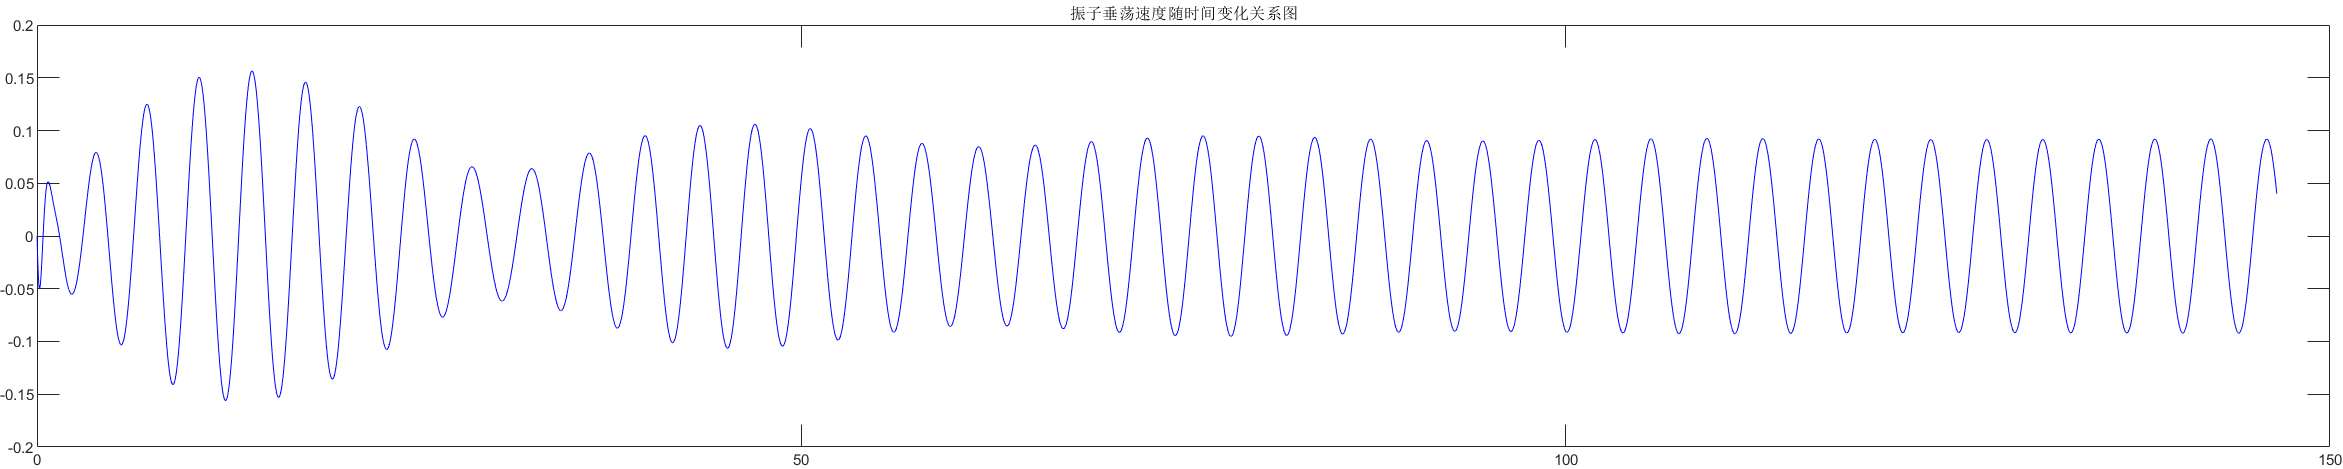
\includegraphics[scale=0.3]{问题3-7.png}
    \caption{振子垂荡速度随时间变化关系图}
\end{figure}
\begin{figure}[H]
    \centering
    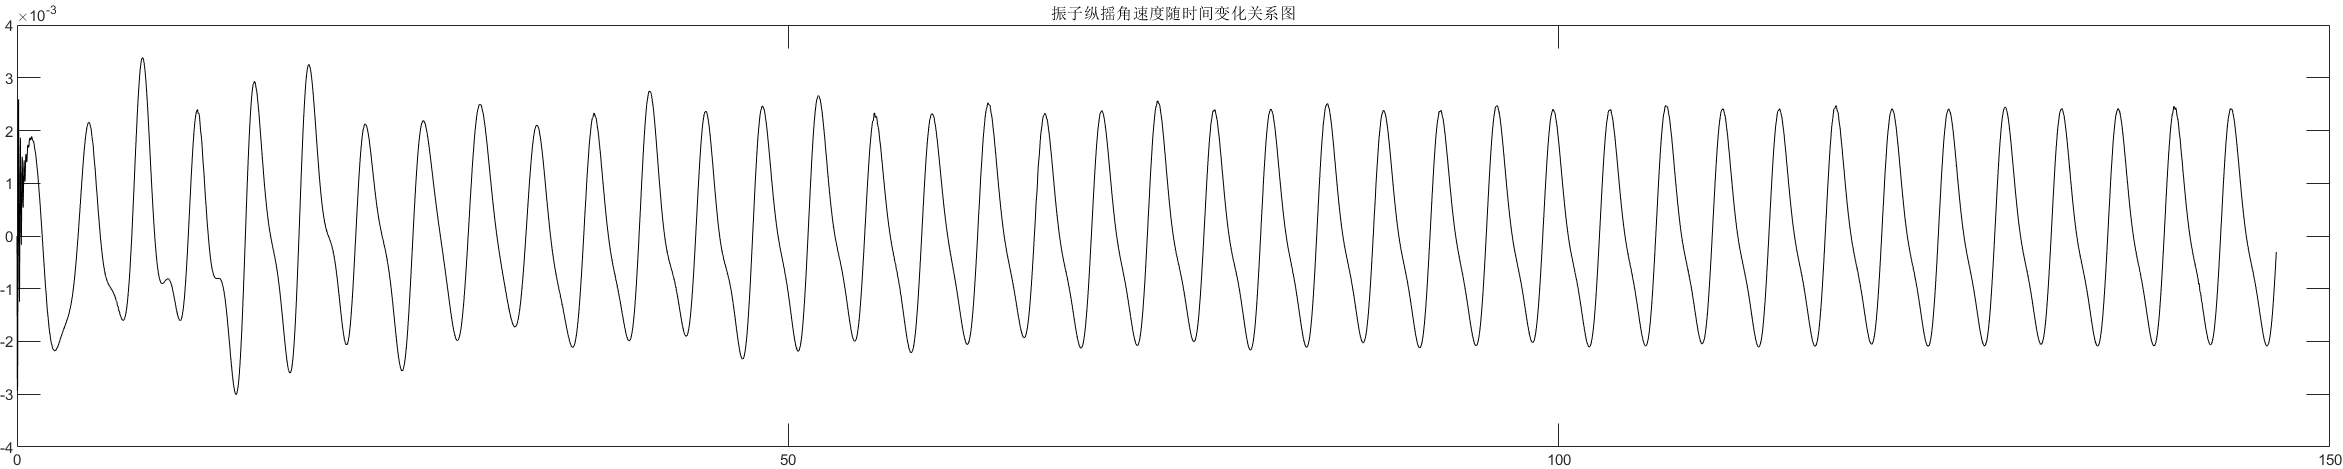
\includegraphics[scale=0.3]{问题3-8.png}
    \caption{振子纵摇角速度随时间变化关系图}
\end{figure}


\section{问题四相关数据及代码}

构建odefun函数
\begin{lstlisting}
    function dxb=odefun_q4(t,xb,etap,etar)%隔离法
    V=(4866+2433)/1025; 
    V1=1/3*pi*0.8; 
    x0=-(V-V1)/pi+1.4;
    z0=x0+0.5-2433*9.8/80000;
    mx=4866;r=1;mz=2433;ro=1025;g=9.8;k=80000;l0=0.5;kr=250000;kh=8890.7;
    w=1.9806;M=1091.099;Jf=7142.493;etax=528.5018;kx=1655.909;f=1760;L=2140;
    J0=5231.83;
    %xb(1)=x;xb(2)=beta;xb(3)=z;xb(4)=alpha;xb(5)=vx;xb(6)=vbeta;xb(7)=vz;xb(8)=valpha;
    dxb=zeros(8,1);
    dxb(1)=xb(5);
    dxb(2)=xb(6);
    dxb(3)=xb(7);
    dxb(4)=xb(8);
    dxb(5)=(mz*g+ro*g*pi*r^2*(x0-xb(1)/cos(xb(2)))+f*cos(w*t)-etax*xb(5)+etap*xb(7)*cos(xb(2)+xb(4))-k*(l0-xb(3))*cos(xb(4)+xb(2)))./(mx+M);
    dxb(6)=(L*cos(w*t)-kx*xb(6)-kh*xb(2)+kr*xb(4)+etar*xb(8))./(J0+Jf);
    dxb(7)=(k*(l0-xb(3))-etap*xb(7)-cos(xb(4)+xb(2))*mz*g)./mz-cos(xb(4)+xb(2))*dxb(5)+sin(xb(4))*1.4*dxb(6);
    dxb(8)=(-kr*xb(4)-etar*xb(8)+sin(xb(4)+xb(2))*mz*g*xb(3))./(mz*xb(3)*xb(3))-sin(xb(4)+xb(2))*dxb(5)-cos(xb(4))*1.4*dxb(6);
    end
\end{lstlisting}

检索及绘图1
\begin{lstlisting}
    etap=[0:5000:100000];
    etar=[0:5000:100000];
    plist=zeros(21,21);%plist_k=zeros(201,21);plist_a=zeros(201,21);
    figure(1);
    for j=1:21
    for i = 1:21
    p=powerp2(etap(i),etar(j));
    plist(i,j)=p;
    %plist_k(i,j)=i;plist_a(i,j)=j;
    scatter3(etap(i),etar(j),p)
    hold on
    end
    end
    [B,IX] = sort(plist(:),'descend');
    [I,J] = ind2sub(size(plist),IX) ;
    scatter3(etap(I(1:80)),etar(J(1:80)),B(1:80),'filled')
    hold off 
    figure(2);
    figure2=scatter(etap(I(1:80)),etar(J(1:80)),'filled');
    [m,im]=max(plist);
    [m2,im2]=max(m);
    i=im(im2);
    j=im2;
    etap_index=etap(i)
    etar_index=etar(j)

    % plot(knp,p,'o-','MarkerSize',3)
    % hold on
    % [b,i]=sort(p);
    % plot(knp(i(end-9:end)),b(end-9:end),'*','MarkerSize',15)
    % max=sum(b(end-9:end))/10;
    % index=sum(knp(i(end-9:end)))/10;

    function p=powerp2(etap,etar)
    V=(4866+2433)/1025; 
    V1=1/3*pi*0.8; 
    x0=-(V-V1)/pi+1.4;
    z0=0.5-2433*9.8/80000;
    b0=0;a0=0;
    w=1.9806;
    x1=0;z1=0;b1=0;a1=0;
    %隔离法
    [~,xz1]=ode45(@(t,xz1)odefun_q4(t,xz1,etap,etar),[0:0.2:40*2*pi/w],[x0;b0;z0;a0;x1;b1;z1;a1]);
    vz=xz1(:,7);
    va=xz1(:,8);
    fix1=fix(20*2*pi/w);fix2=fix(40*2*pi/w);
    square=abs(vz(fix1*5:fix2*5)).^2*etap+abs(va(fix1*5:fix2*5)).^2*etar; %%取20-60s稳定后的值来计算平均做功
    area=1:(-fix1+fix2)*5;
    for i=1:-fix1*5+fix2*5
    area(1,i)=(square(i,1)+square(i+1,1))*0.1;
    end
    p=sum(area)/(20*2*pi/w);
    end
\end{lstlisting}

检索及绘图2
\begin{lstlisting}
    etap=[63420:0.5:63430];
    etar=[99990:0.5:100000];
    plist=zeros(21,21);
    figure(1);
    for j=1:21
    for i = 1:21
    p=powerp2(etap(i),etar(j));
    plist(i,j)=p;
    %plist_k(i,j)=i;plist_a(i,j)=j;
    scatter3(etap(i),etar(j),p)
    hold on
    end
    end

    [B,IX] = sort(plist(:),'descend');
    [I,J] = ind2sub(size(plist),IX) ;
    scatter3(etap(I(1:20)),etar(J(1:20)),B(1:20),'filled')
    hold off 

    figure(2);
    figure2=scatter(etap(I(1:20)),etar(J(1:20)),'filled');
    [m,im]=max(plist);
    [m2,im2]=max(m);
    i=im(im2);
    j=im2;
    etap_index=etap(i)
    etar_index=etar(j)

    % plot(knp,p,'o-','MarkerSize',3)
    % hold on
    % [b,i]=sort(p);
    % plot(knp(i(end-9:end)),b(end-9:end),'*','MarkerSize',15)
    % max=sum(b(end-9:end))/10;
    % index=sum(knp(i(end-9:end)))/10;

    function p=powerp2(etap,etar)
    V=(4866+2433)/1025; 
    V1=1/3*pi*0.8; 
    x0=-(V-V1)/pi+1.4;
    z0=0.5-2433*9.8/80000;
    b0=0;a0=0;
    w=1.9806;
    x1=0;z1=0;b1=0;a1=0;
    %隔离法
    [~,xz1]=ode45(@(t,xz1)odefun_q4(t,xz1,etap,etar),[0:0.2:40*2*pi/w],[x0;b0;z0;a0;x1;b1;z1;a1]);
    vz=xz1(:,7);
    va=xz1(:,8);
    fix1=fix(20*2*pi/w);fix2=fix(40*2*pi/w);
    square=abs(vz(fix1*5:fix2*5)).^2*etap+abs(va(fix1*5:fix2*5)).^2*etar; %%取20-60s稳定后的值来计算平均做功
    area=1:(-fix1+fix2)*5;
    for i=1:-fix1*5+fix2*5
    area(1,i)=(square(i,1)+square(i+1,1))*0.1;
    end
    p=sum(area)/(20*2*pi/w);
    end
\end{lstlisting}
\end{document}


